%----------------------------------------------------------------------------------------
%	CHAPTER - DEVELOPMENT
%----------------------------------------------------------------------------------------

\chapter{Development}

\label{ChapterDevelopment}

% ################################################################
\definecolor{bluekeywords}{rgb}{0,0,1}
\definecolor{greencomments}{rgb}{0,0.5,0}
\definecolor{redstrings}{rgb}{0.64,0.08,0.08}
\definecolor{xmlcomments}{rgb}{0.5,0.5,0.5}
\definecolor{types}{rgb}{0.17,0.57,0.68}

\lstset{language=[Sharp]C,
	captionpos=b,
	%numbers=left, %Nummerierung
	%numberstyle=\tiny, % kleine Zeilennummern
	frame=lines, % Oberhalb und unterhalb des Listings ist eine Linie
	showspaces=false,
	showtabs=false,
	breaklines=true,
	showstringspaces=false,
	breakatwhitespace=true,
	escapeinside={(*@}{@*)},
	commentstyle=\color{greencomments},
	morekeywords={partial, var, value, get, set},
	keywordstyle=\color{bluekeywords},
	stringstyle=\color{redstrings},
	basicstyle=\ttfamily\small,
}
% ################################################################

%----------------------------------------------------------------------------------------
%	SECTION 1
%----------------------------------------------------------------------------------------

\section{Introduction}

The \textit{Development} phase, as defined by \cite{Vaishnavi2008} and \cite{Hevner2010}, comes after the \textit{Suggestion} of a design and focuses on the further development and implementation of the design. The outcome of this chapter is the requirement for the subsequent \textit{Evaluation} chapter. This is a crucial step in answering \gls{srq} 4 since the to be achieved benefits over the traditional approaches have only been of theoretical nature so far, but are not tested for their feasibility yet. \cite{Vaishnavi2008} see different techniques on how the implementation can look like, depending on the to be constructed artifact. For this thesis, the development of a prototype application in \gls{vr} has been chosen. In a first step, the technical setup is defined, before the architecture and data model for the prototype are discussed. Following that, the actual implementation of the different views and navigations are covered with a conclusion at the end. \newline
Building up on this, the \textit{Evaluation} phase will then be discussed in chapter \ref{ChapterEvaluation}.


%----------------------------------------------------------------------------------------
%	SECTION 2
%----------------------------------------------------------------------------------------

\section{Technical Setup}

The technical setup chapter gives a description and explanation for the selection of the individual components that are used for the development of the prototype application. It can be distinguished between Hardware and Software components that are discussed in their respective sub-chapters.


%-----------------------------------
%	SUBSECTION 1
%-----------------------------------
\subsection{Hardware}

The in the literature review discussed different methods for user input as part of \gls{srq} 2 have been summarized in table \ref{tbl:methodscomparison}. For the selection of the right \gls{vr} device, this conclusion was considered for the evaluation. While for the \textit{Travel} aspect only three methods (including the option for no travel at all) have been discussed:

\textbf{No travelling option:}
By looking at \gls{mdg} 2 that defines the user to be part of the \gls{ve} and thus is able to 'travel' around the visualisations, the third option would violate this design goal and thus is no viable option.

\textbf{Full Body Tracking:}
While it allows for free movement within \gls{ve}, it is lacking accuracy and only works from one angle. This can be effectively used if a static display in one direction is used which updates the data that it displays. With an implementation of the 'multiples linked views' concept however, one angle will not be enough anymore.

\textbf{360° Motion Tracking:}
Compared to 'Full Body Tracking', the '360° Motion Tracking' provides much better accuracy and allows for spatial positioning in all three axis, which strongly supports \gls{mdg} 2.


This leads to a first conclusion for '360° Motion Tracking' which is the only methods for \textit{Travel} that fulfils all requirements of the design goals. For \textit{Selection} (and \textit{Manipulation}), some more methods had been discussed:

\textbf{No selection/manipulation option:}
The option for no input method cannot be considered as the application would then provide no interaction at all and thus violate \gls{mdg} 1 that requires a high interactivity with tightly coupled actions/reactions.

\textbf{Hand Gestures:}
While 'Hand Gestures' offer a very high familiarity, they have a limited tracking area and become less accurate with faster movements. Although the latter is not of that importance, the limited tracking area can become problematic with the different views, especially since the supporting views are placed in the centre of where the user is looking at.

\textbf{Gesture Controllers:}
TODO: tbd

\textbf{Speech Recognition:}
This methods requires a silent area and good pronunciation of one of the supported official languages, as dialects can be quite problematic. While it allows for some very interesting, more complex queries such as "Show me all transactions in the last seven days over CHF 100.", it rather can be seen as a supportive input method, but not as the main input method.

\textbf{Physical Placement of Objects:}
While the 'Physical Placement of Objects' would be the most realistic and immersive option, it can be considered as to expensive and also too difficult to build as for this design goal not only some buttons and knobs would need to be built, but also fully dynamic charts and tables.


It can be concluded, that the 'Gesture Controllers' have the highest fit, and also work very well together with the '360° Motion Tracking'. Speech Recognition can provide some interesting support-functionalities that should be looked at in future research. \newline
This combination of input methods are best met with the HTC Vive (\url{https://www.vive.com/}) that was unveiled by HTC in early 2016. The bundle consists of a \gls{hmd}, two gesture controllers (as explained in Chapter \ref{SubSubSectionGestureControllers}) and two so called 'Lighthouses' (as explained in Chapter \ref{360MotionTracking}) that when set up in opposite corner allow for a full motion tracking.


%-----------------------------------
%	SUBSECTION 2
%-----------------------------------

\subsection{Software}

All used software for the development of the \gls{vr} prototype is summarised and described in the following sub-chapters.


\subsubsection{Game Engine}
At the foundation, the multi-platform game engine and development toolkit 'Unity 3D' is used. It offers the option to not only develop 2D, but also 3D applications that can be run in \gls{vr}. It is used for the actual design of the \gls{ve}, and the placement and configuration of 3D objects.

\textbf{Software:} Unity 3D \newline
\textbf{Version:} 5.5.0f3 \newline
\textbf{Publisher:} \cite{Unity2016} \newline
\textbf{Link:} \url{http://unity3d.com/}


\subsubsection{Game Engine Plugins}
For the integration of the \gls{sdk} to access the specific methods and functions of the HTC Vive, the SteamVR plugin for Unity is used. In addition to this, \gls{vrtk} will be used as a toolkit to rely on 'semi-standardised' ways for certain \gls{vr}-specific interactions and functions in Unity 3D. Even though the HTC Vive has been chosen for the hardware part, due to the usage of the SteamVR plugin and the \gls{vrtk}, only little to none changes should be required in order to have the prototype application also run other supported hardware such as the Oculus Rift, since both of them support multiple \glspl{hmd}.

\textbf{Software:} SteamVR Plugin \newline
\textbf{Version:} 1.1.1 \newline
\textbf{Publisher:} \cite{Valve2016a} \newline
\textbf{Link:} \url{https://www.assetstore.unity3d.com/en/#!/content/32647}

\textbf{Software:} \gls{vrtk} - Virtual Reality Toolkit \newline
\textbf{Version:} 3.0.0 \newline
\textbf{Publisher:} \cite{Sysdia2017} \newline
\textbf{Link:} \url{https://www.assetstore.unity3d.com/en/#!/content/64131} \newline
\textbf{Link:} \url{https://vrtoolkit.readme.io/}


\subsubsection{\gls{ide}}
Microsoft Visual Studio Community 2015 from  is used for the development of the Unity Scripts in the programming language C\#. These scripts handle and manage the whole \gls{ve} by triggering interactions of the 3D objects defined and placed in Unity 3D.

\textbf{Software:} Microsoft Visual Studio Community \newline
\textbf{Version:} 2015 \newline
\textbf{Publisher:} \cite{Microsoft2015} \newline
\textbf{Link:} \url{https://www.microsoft.com/en-us/download/details.aspx?id=48146}
 

\subsubsection{3D Graphics}

Finally, for the design of custom 3D models as representations of the category icons as shown in Figure \ref{fig:categoriesicons} in Chapter \ref{SubSectionCategoriesFiltering}, the  open-source 3D computer graphics software Blender is used. The exported models are fully compatible with Unity 3D and can be seamlessly imported and used.

\textbf{Software:} Blender \newline
\textbf{Version:} 2.78a \newline
\textbf{Publisher:} \cite{Blender2016} \newline
\textbf{Link:} \url{https://www.blender.org/}


%----------------------------------------------------------------------------------------
%	SECTION 3
%----------------------------------------------------------------------------------------

\section{Architecture and Design}

A key part of the prototype development is the (software) architecture as well as the overall (software) design. In the following sub-chapters, several aspects of the architecture and design are discussed, which includes the general architecture, the data model, and the code structure.


%-----------------------------------
%	SUBSECTION 1
%-----------------------------------
\subsection{General Architecture}

Figure \ref{fig:steamvrselected} shows the general architecture of the Steam VR plugin for Unity 3D and how it acts as a wrapper for multiple different \glspl{hmd} that can be communicated with. The \gls{vrtk} itself then is part of the software itself as its scripts are used for the application and can also be extended to provide additional functionality that is not offered from the base toolkit. The base data set which is available as a .CSV file is accessed from within the software and stored inside multiple different data objects that are discussed in more detail in the following 'Data Model' chapter.

\begin{figure}[h]
	\begin{center}
		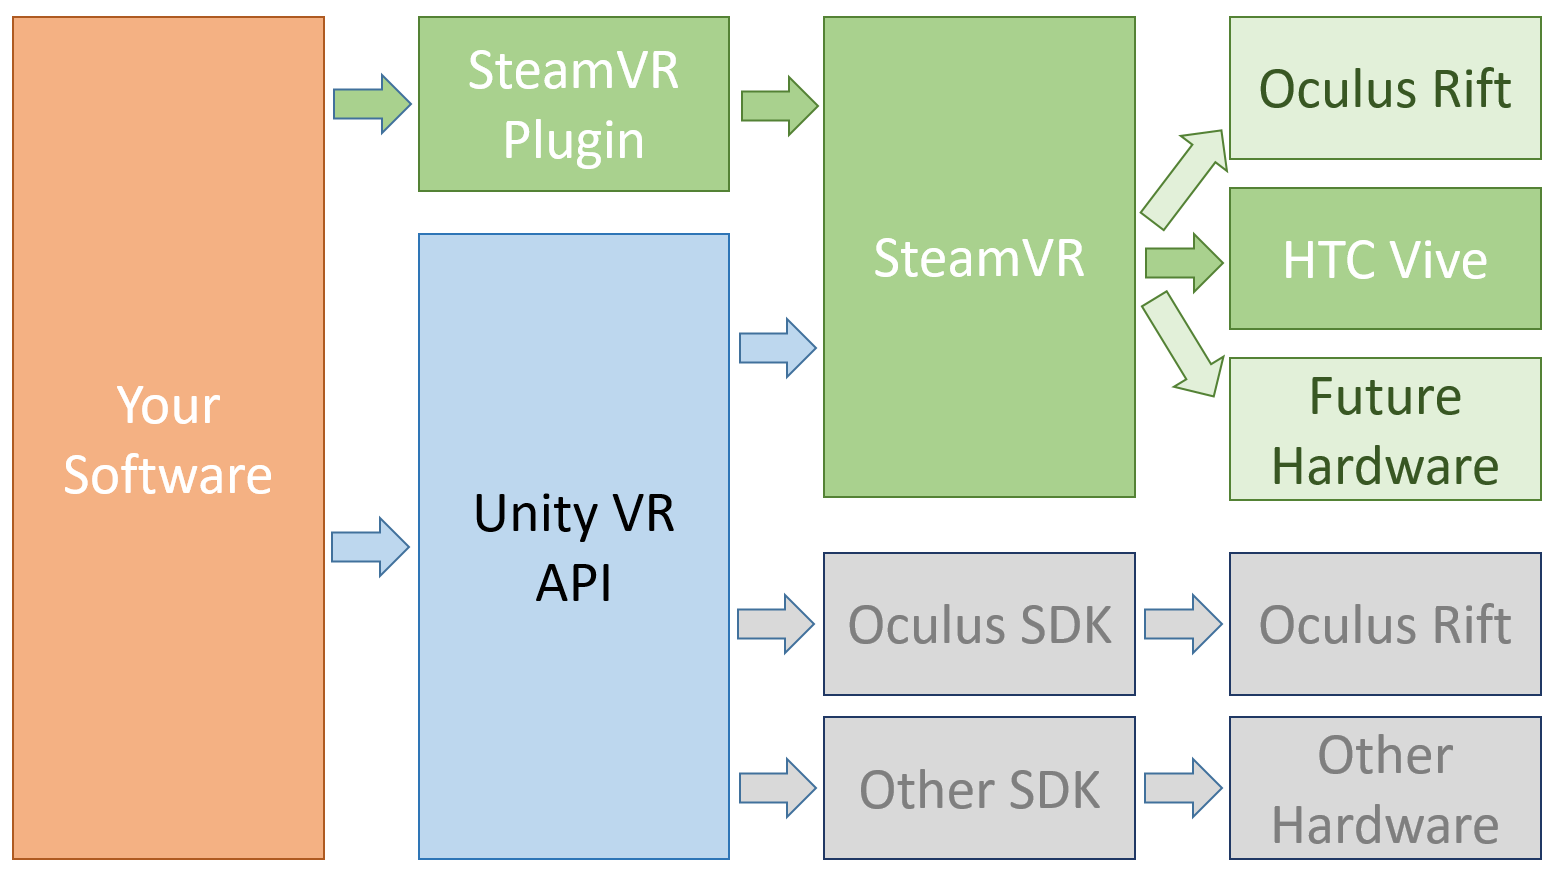
\includegraphics[width=14cm]{03_Figures/04_Valve/OpenVR_SteamVR_selected.png}
		\caption[Steam VR Unity Plugin]{Steam VR Unity Plugin (adopted from \cite{Valve2016})}
		\label{fig:steamvrselected}
	\end{center}
\end{figure}



%-----------------------------------
%	SUBSECTION 2
%-----------------------------------

\subsection{Data Model}

One of the main challenges is to get reasonable performance while working with a not so small data set (600+ entries as shown in Appendix \ref{AppendixA}) that can be filtered not only by year/month/day but also by several different categories atop of that. In order to not always filter through the whole data set, it will be split up in smaller parts that contain only data for a specific month in a specific year. While reading in the CSV file, multiple instances of the \texttt{[System.Data.DataTable]} class are created and stored with the unique key \texttt{[$<$year$>$-$<$month$>$]} in a \texttt{[System.Collections.Generic.Dictionary]} which is the C\# equivalent of a HashMap in Java. For the filtering of the DataTable, the \texttt{[System.Data.DataView]} class is used which itself does not store data but represents a connected view of a DataTable. While this already helps with the performance, as soon as the category filtering comes in place it still is relatively slow as all twelve months need to be updated. \newline
To at least partially address this problem, a caching of the filtered data for the bar charts and table has been considered. For this, another unique key had to be defined in the form of \texttt{[$<$year$>$-$<$month$>$-$<$day$>$-$<$binaryCategory$>$]}. The \texttt{binaryCategory} is a binary state representation of all \textbf{eleven} categories where each one of them is either represented as a '0' (inactive) or a '1' (active). Following are some example to indicate how certain situations can be represented:
\begin{itemize}[noitemsep,nolistsep]
	\item \texttt{2016-0-0-00000000000} \textit{(only year selected and all categories inactive)}
	\item \texttt{2016-3-0-11111111111} \textit{(single month selected and all categories active)}
	\item \texttt{2016-8-27-11100010101} \textit{(selection of a specific day with different category states)}
\end{itemize}
With eleven categories, over 2'048 different combinations can be made across them. If this is considered for a whole year (365 days) there are a staggering amount of 747'520 different key-combinations, which makes it impractical to try to pre-cache every single combination. Due to this an on-demand cache is implemented to at least massively reduce the loading times of previously selected combinations. Listing \ref{lst:csharpdictionarydefinition} shows all definitions for the different containers that hold the information during runtime. \texttt{dataTableDict} stores the different \texttt{DataTable}s per month, \texttt{chartValuesDict} and \texttt{chartLabelsDict} contain the labels and values for all bar charts with their long unique key, and finally \texttt{tableRowsDict} which helds the information for the table again with the long unique key. All these attributes are defined in the \texttt{DataViewManager.cs} class that is referenced in the \texttt{SceneManager.cs} class which is a Singleton instance and thus is guaranteed to only exist once in runtime and is also always accessible from any other script.
\begin{lstlisting}[caption={Dictionary definitions for data storage during runtime}, label={lst:csharpdictionarydefinition}]
public Dictionary<string, DataTable> dataTableDict;
private Dictionary<string, float[]> chartValuesDict;
private Dictionary<string, string[]> chartLabelsDict;
private Dictionary<string, List<string[]>> tableRowsDict;
\end{lstlisting}


%-----------------------------------
%	SUBSECTION 3
%-----------------------------------

\subsection{Code Structure}

It is important to have an effective and clean code structure that reflects the different layers which all together become the software itself. The following Figure \ref{fig:unitycodestructure} shows the project structure in Unity 3D while Table \ref{tbl:codestructuredesc} explains this in more detail. The structure follows some best practices that are also applied in SteamVR and \gls{vrtk}.
\begin{figure}[h]
	\begin{center}
		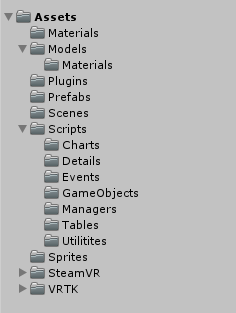
\includegraphics[width=7cm]{03_Figures/08_Development/CodeStructure.png}
		\caption{Prototype project structure in Unity 3D}
		\label{fig:unitycodestructure}
	\end{center}
\end{figure}


\begin{longtable}{ | p{3cm} | p{11cm} |}
	\hline
	\textbf{Folder} & \textbf{Description} \\
	\hline
	\endfirsthead % Line(s) to appear as head of the table on the first page
	\multicolumn{2}{c}%
	{\tablename\ \thetable\ -- \textit{Continued from previous page}} \\
	\hline
	\textbf{Folder} & \textbf{Description} \\
	\hline
	\endhead % Line(s) to appear at top of every page (except first)
	\hline
	\multicolumn{2}{r}{\textit{Continued on next page}} \\
	\endfoot % Last line(s) to appear at the bottom of every page (except last)
	\endlastfoot % Last line(s) to appear at the end of the table
	\hline
		\textbf{Assets} &
		This is the base-folder which is given by Unity 3D itself. It contains all files that are either required or created by the developer. \\
	\hline
		Materials &
		The Materials folder contains material (\texttt{*.mat}) files that can be applied to 2D/3D objects. \\
	\hline
		Models &
		In this folder, all models created in Blender (\texttt{*.blend}) are stored which can be dragged into the 3D scene. \\
	\hline
		\textrightarrow{} Materials &
		Contains all model-specific material (\texttt{*.mat}) files that are created in Blender. \\
	\hline
		Plugins &
		Additional C\# plugins (\texttt{*.dll}) are put here such as System.Data.dll which allows the processing and manipulation of data files. \\
	\hline
		Prefabs &
		In this folder, fully configured GameObjects can be stored (\texttt{*.prefab}) and instantiated multiple times. All instances inherit the base configuration and changes can be applied to all of them very easily. The individual bars of the bar chart are an example of such a prefab. \\
	\hline
		Scenes &
		Within one Unity project, there can be multiple scenes (\texttt{*.unity}), which can be seen some kind of broken down parts of bigger applications where multiple different locations are available. In this prototype there is only a single scene used. \\
	\hline
		Scripts &
		The base folder for all C\# scripts (\texttt{*.cs}) that are used. \\
	\hline
		\textrightarrow{} Charts &
		Contains all scripts that are related to the functionality of the bar charts. \\
	\hline
		\textrightarrow{} Details &
		All scripts related to the detail view where all information about a financial transaction are shown. \\
	\hline
		\textrightarrow{} Events &
		Custom events that can be triggered from the gesture controllers are located here. \\
	\hline
		\textrightarrow{} GameObjects &
		Scripts related to specific game objects (e.g. the category icons) are stored in this folder. \\
	\hline
		\textrightarrow{} Managers &
		Contains two manager classes that hold together the whole information of the running scene and the stored/cached data. \\
	\hline
		\textrightarrow{} Tables &
		All scripts that are related to the table which shows a list of financial transactions \\
	\hline
		\textrightarrow{} Utilities &
		All other utility classes such as a unified Debugging/Logging. \\
	\hline
		Sprites &
		In this folder any kind of images (e.g. \texttt{*.png}) are stored that are used within the application, such as the threshold line for the bar charts. \\
	\hline
		SteamVR &
		Here all folders and files from the SteamVR plugin are copied to. It also contains certain prefabs that control the \gls{hmd} and gesture controllers. \\
	\hline
		\gls{vrtk} &
		Similar to the SteamVR folder, all scripts and prefabs from \gls{vrtk} are located under this folder. \\
	\hline
	\caption{Explanation of prototype project structure in Unity 3D}
	\label{tbl:codestructuredesc}
\end{longtable}


%----------------------------------------------------------------------------------------
%	SECTION 4
%----------------------------------------------------------------------------------------

\section{Implementation of Views and Interaction}

In this chapter, an overview of all the views and their usage is provided, as well the interactions between them is mentioned.

%-----------------------------------
%	SUBSECTION 1
%-----------------------------------
\subsection{Views / UI}

The following list of views refers back to the Suggestion chapter where the Navigation Map (Figure \ref{fig:navigationmap}) and Interaction Map (Figure \ref{fig:interactionmap}) are described. For each view a short explanation about its purpose is provided, alongside some design aspects from the development, and a screenshot that shows the view of final prototype application. Figure \ref{fig:unityoverview} gives an overview over the whole scene in Unity 3D where all the different views are arranged almost in a circle around the centre where the user will be spawning.

\begin{figure}[h]
	\begin{center}
		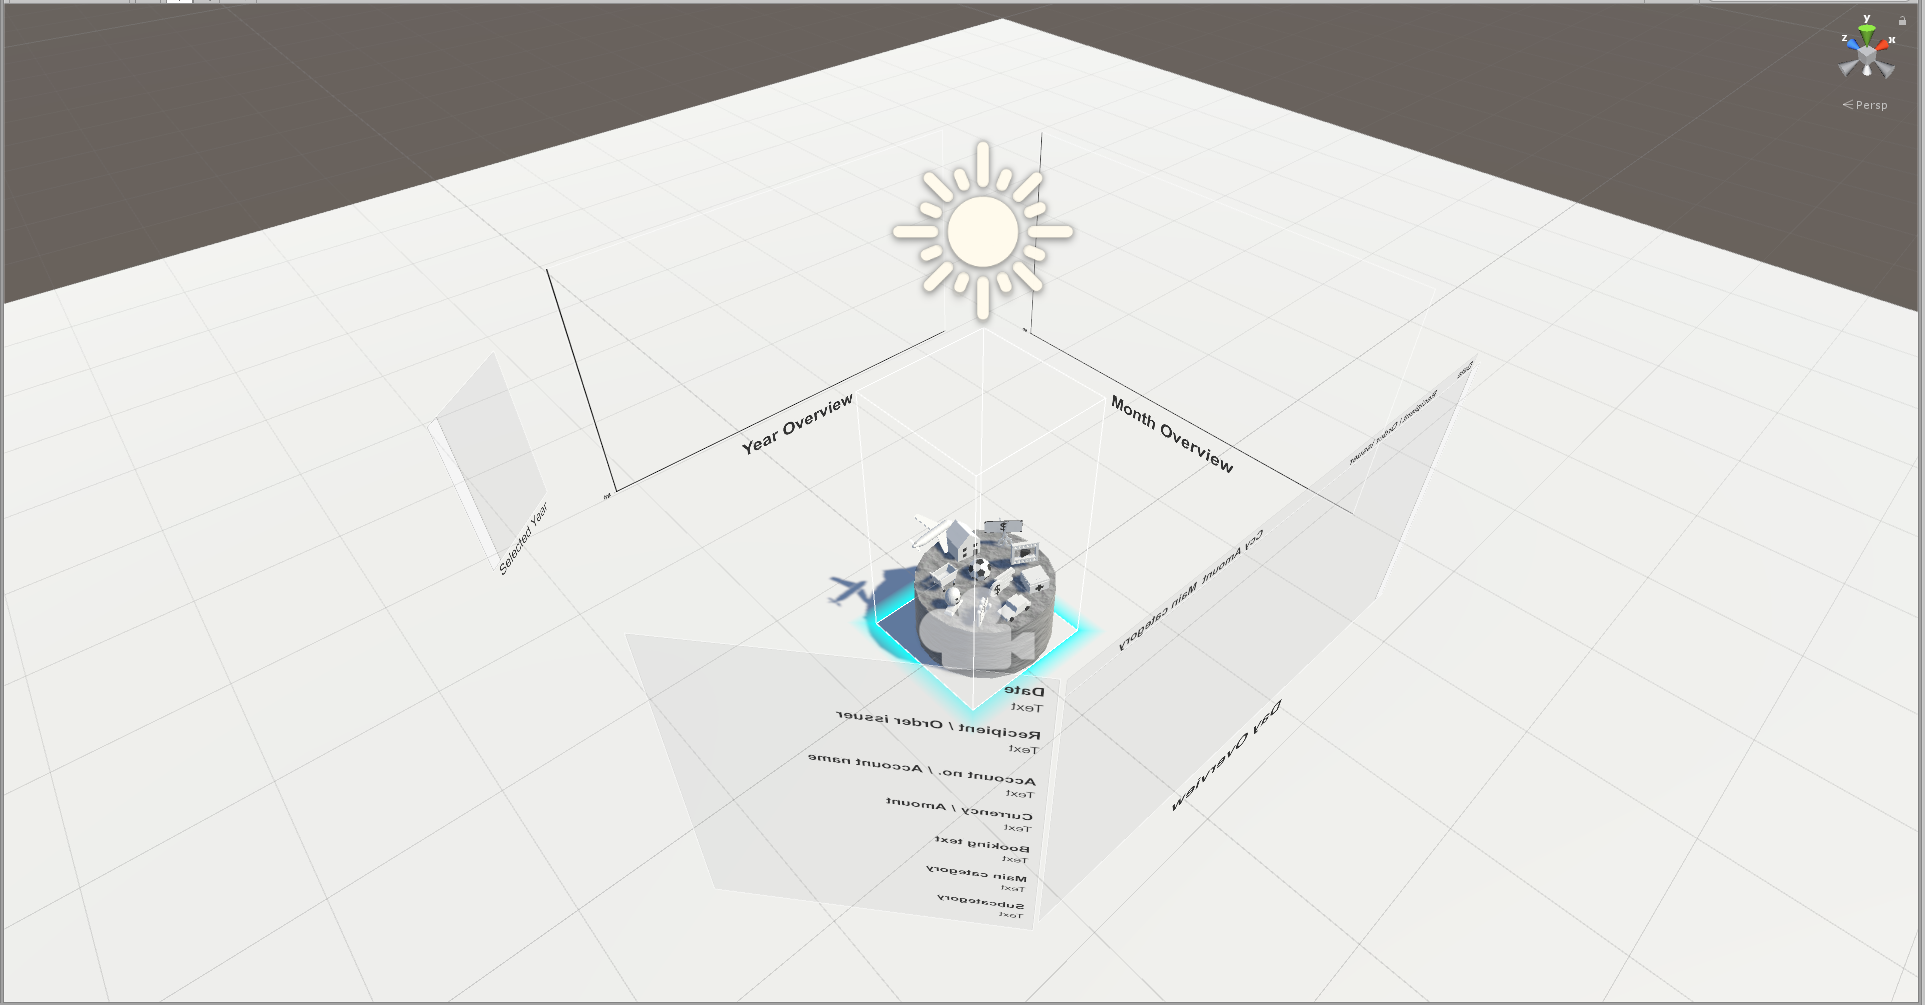
\includegraphics[width=12cm]{03_Figures/08_Development/Unity_Overview.png}
		\caption{Scene Overview in Unity 3D}
		\label{fig:unityoverview}
	\end{center}
\end{figure}

%-----------------------------------
%	SUBSUBSECTION 1
%-----------------------------------
\subsubsection{View 1: Year Overview}

This is the first view the user will see when he spawns in the \gls{ve}, it is located directly in front of him.

\textbf{Purpose of view:} It provides a comprehensive overview over the situation of the financial expenses. Each category has its own expenses threshold defined which defines on what amount the vertical threshold line is drawn. This can be seen in Figure \ref{fig:unityview1} where the threshold is set to 3'300. If the total expenses of a month exceed the threshold, the amount of the bar above the line is in red colour compared to the rest below the line which is in green colour. This gives a very fast indication to the user in which months more money was spent than planned. When a single month is selected, the corresponding bar starts to flash. This allows for a better visual connection between the two charts than just relying on the label below them, which should increase the effectiveness of the "multiple linked views" concept. The bar chart further only includes the categories (and thresholds) that have been activated in view 3.

\textbf{Possible Interaction:} Selecting a bar to...
\begin{itemize}[noitemsep,nolistsep]
	\item see the month overview bar chart (Path 3)
	\item see a list of all financial transactions for that month (Path 4)
\end{itemize}

\begin{figure}[h]
	\begin{center}
		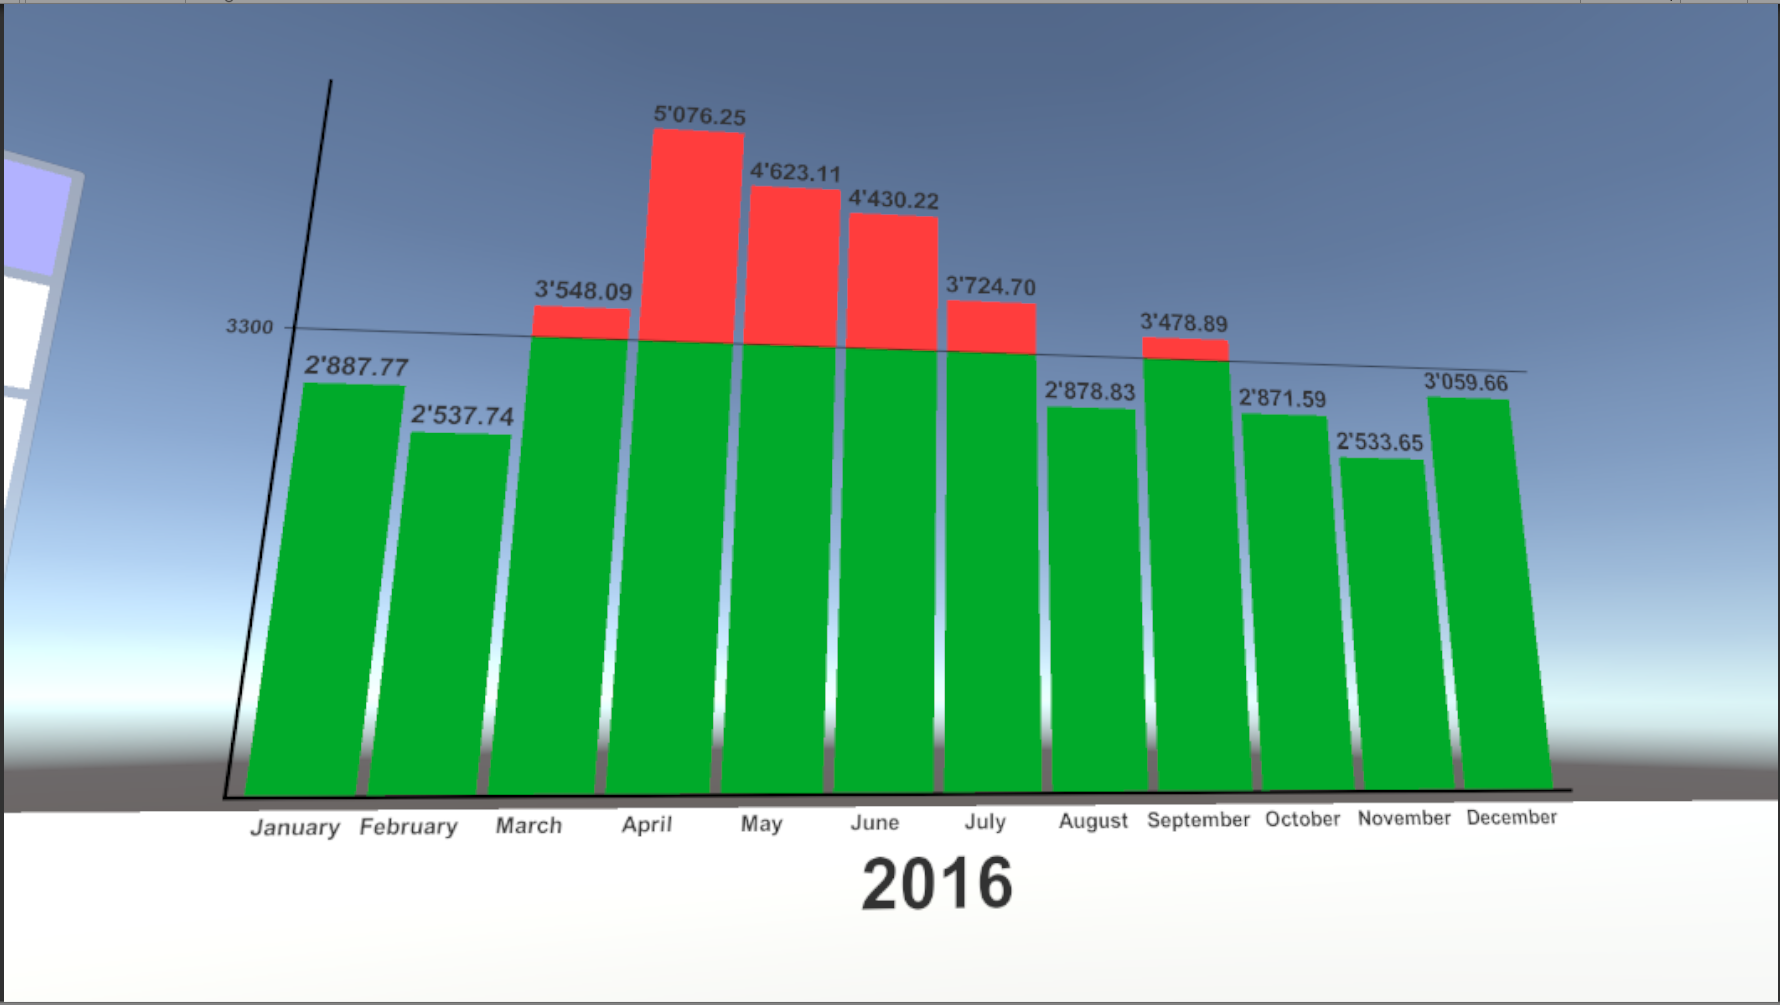
\includegraphics[width=12cm]{03_Figures/08_Development/View1_YearOverview.png}
		\caption{View 1: Year Overview (live in \gls{vr})}
		\label{fig:unityview1}
	\end{center}
\end{figure}


%-----------------------------------
%	SUBSUBSECTION 2
%-----------------------------------
\subsubsection{View 2: Month Overview}

To the right of the year overview (View 1), the month overview can be found. It initially is empty until a month is selected in the year overview.

\textbf{Purpose of view:} Contrary to the year overview, the individual days do not indicate their own total amount of expenses, but they rather stack up with all the previous expenses from that month. This gives the unique insight on which day exactly the threshold had been exceeded. This can be seen very nicely in Figure \ref{fig:unityview2} where the threshold of 3'330 was exceeded on June 21st. To not overload the view with too many numbers, they are only shown when there was a change compared to the previous day. Like the month overview, when a single day is selected, the bar starts flashing for an assisted visual connection. Again, this bar chart only includes the categories (and thresholds) that have been activated in view 3.

\textbf{Possible Interaction:} Selecting a bar to...
\begin{itemize}[noitemsep,nolistsep]
	\item see a list of all financial transactions for that day (Path 4)
\end{itemize}

\begin{figure}[h]
	\begin{center}
		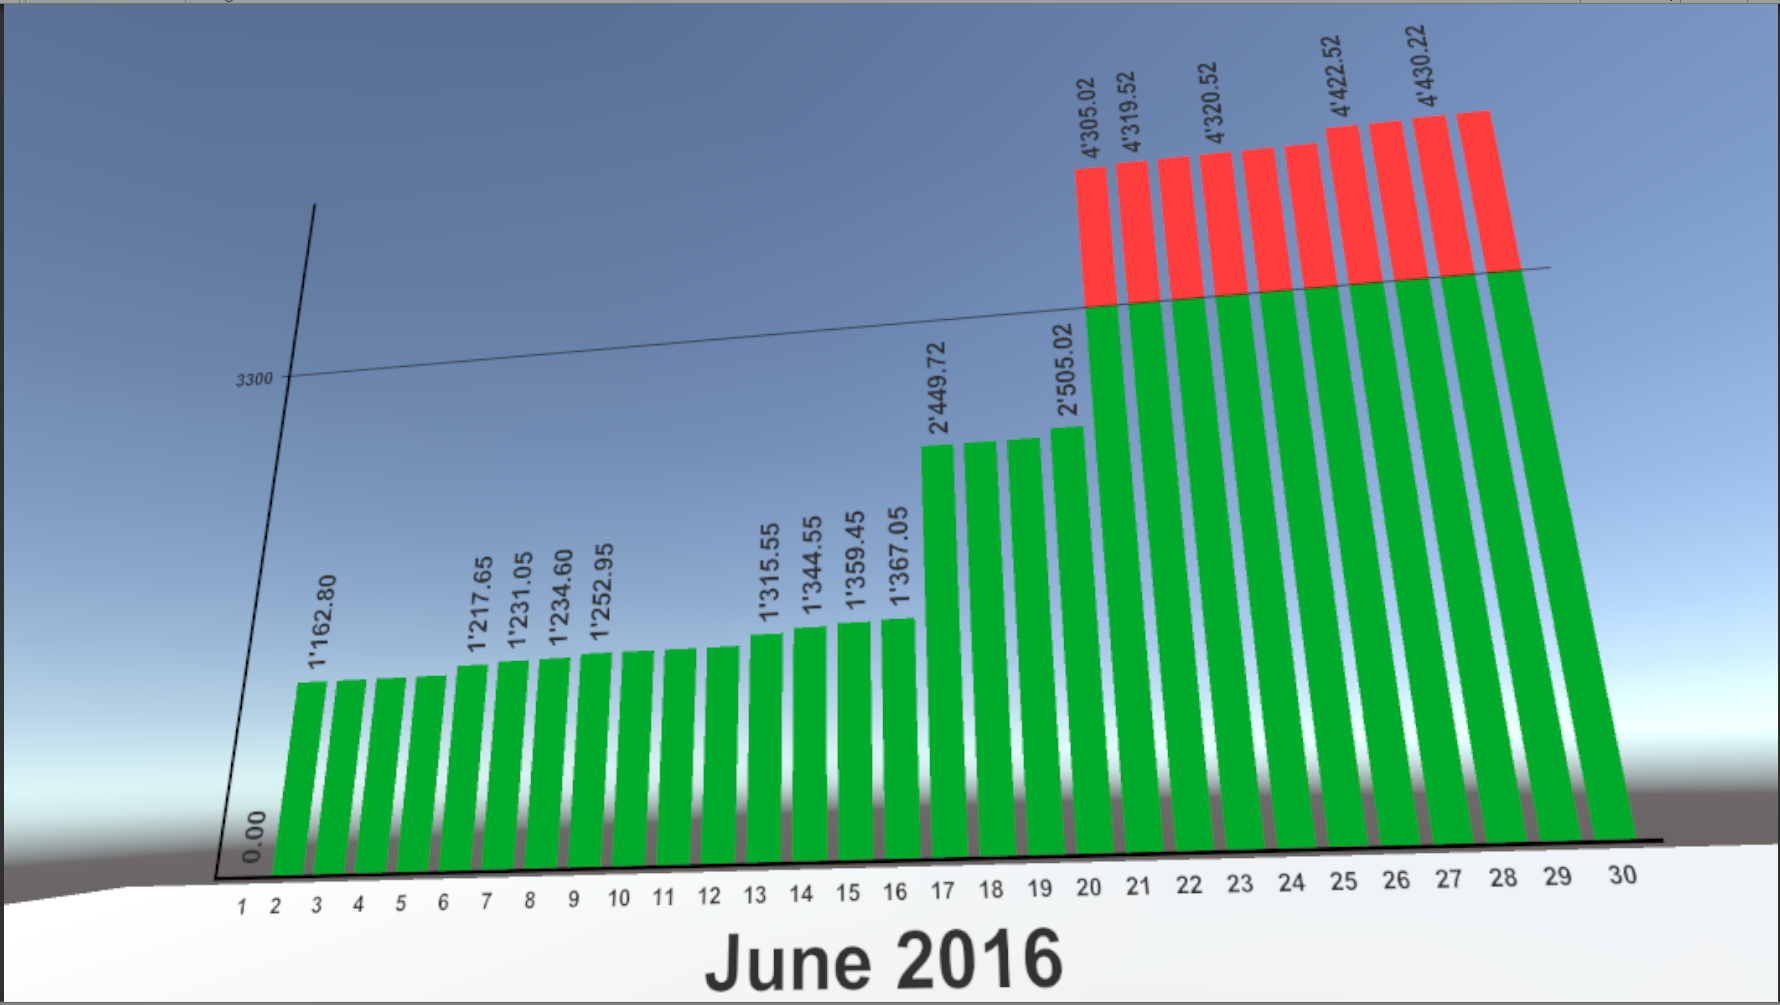
\includegraphics[width=12cm]{03_Figures/08_Development/View2_MonthOverview.png}
		\caption{View 2: Month Overview (live in \gls{vr})}
		\label{fig:unityview2}
	\end{center}
\end{figure}


%-----------------------------------
%	SUBSUBSECTION 3
%-----------------------------------
\subsubsection{View 3: Year Selection}

To the left of the year overview (View 1), the year selection screen is shown in a small scrollable window. 

\textbf{Purpose of view:} The purpose of this small window is to allow the user to view the data from different years and not only the most recent one, which is automatically pre-selected. The list is dynamically populated based on the CSV data source and can due to the scrolling functionality show many more than just a handful of years. By changing the selected year, all other data views will be reset and only the year overview gets populated again with the data from the selected year.

\textbf{Possible Interaction:} Selecting a year to...
\begin{itemize}[noitemsep,nolistsep]
	\item see the year overview bar chart (Path 1)
	\item clear the month overview bar chart (Path 2)
	\item clear the table with financial transactions (Path 4)
\end{itemize}

\begin{figure}[h]
	\begin{center}
		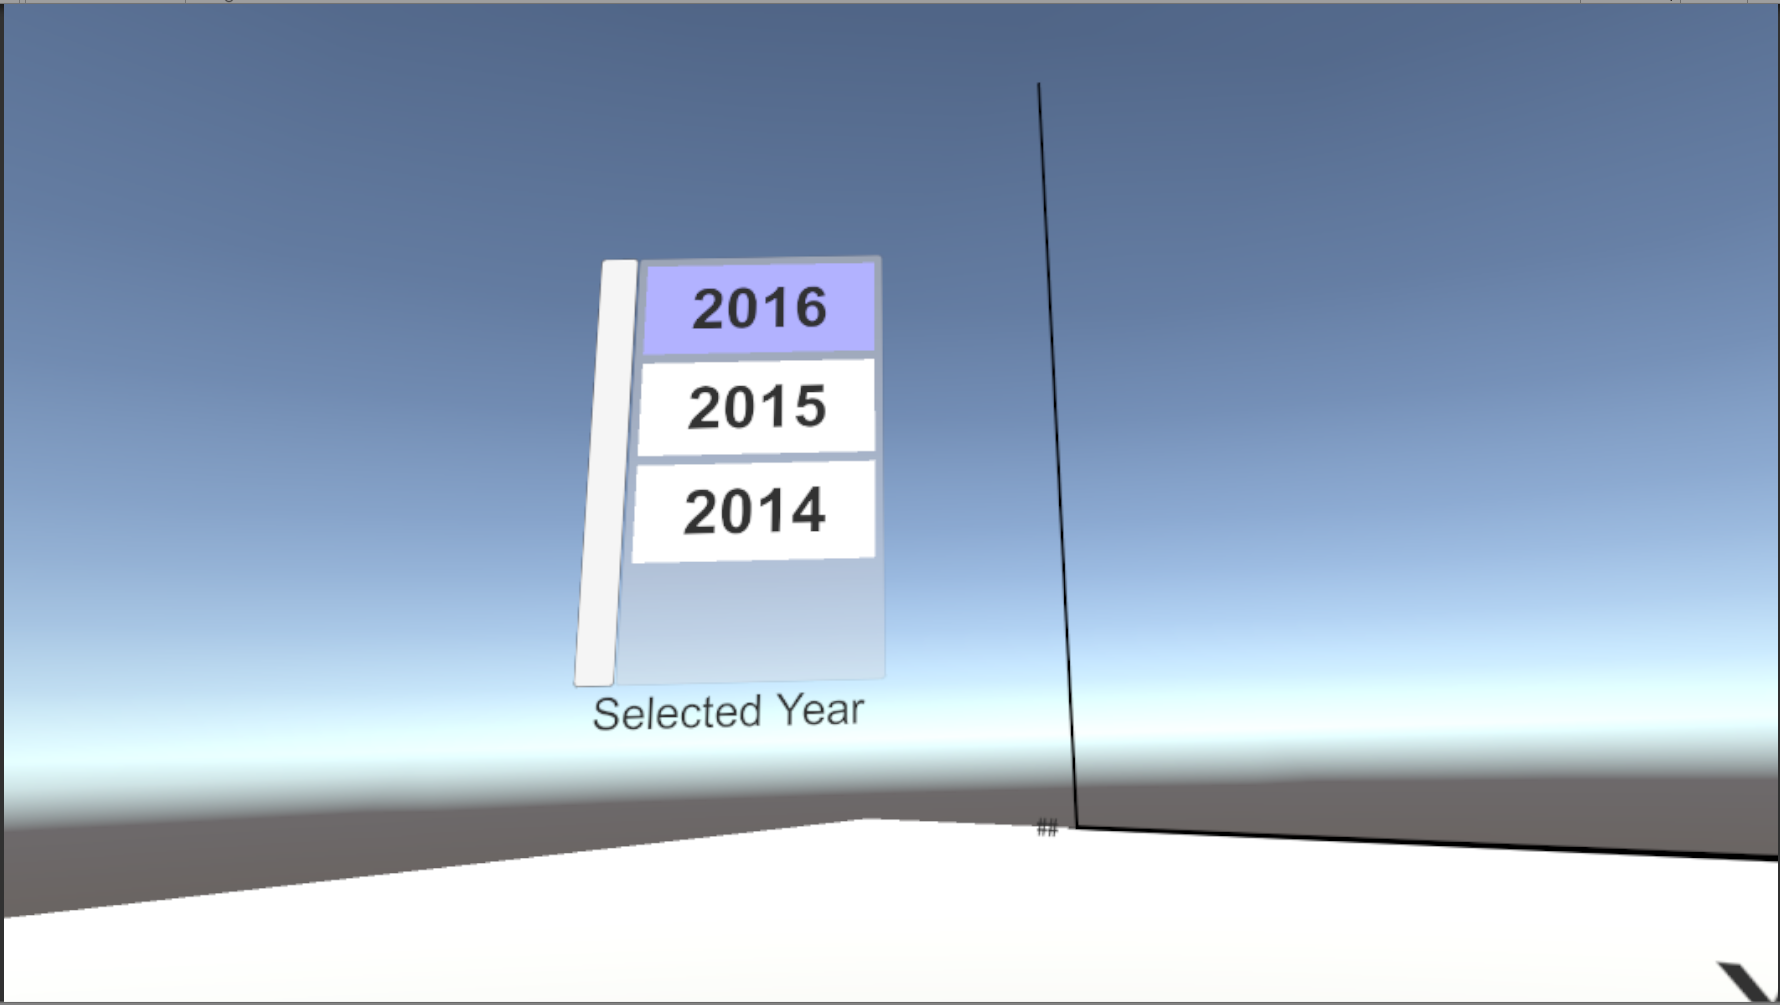
\includegraphics[width=12cm]{03_Figures/08_Development/View3_YearSelection.png}
		\caption{View 3: Year Selection (live in \gls{vr})}
		\label{fig:unityview3}
	\end{center}
\end{figure}


%-----------------------------------
%	SUBSUBSECTION 4
%-----------------------------------
\subsubsection{View 4: Categories Filtering}

Right in front of the user, a bit below eye sight is some kind of a pedestal on which the eleven category icons from Figure \ref{fig:categoriesicons} are represented as 3D models. 

\textbf{Purpose of view:} Changing the selection of the categories should be as close to the user as possible but still not block his view on all the different charts and tables. Therefore it has been located right in front of him on a bit a lower height. Each category object can be in one of three different states: When the category is inactive and thus not considered for being displayed in any of the charts or table, then the object is represented in \textbf{white colour}. When the category is activated and the corresponding transactions are included in the other views, the object is shown in \textbf{green colour}. Due to the increased computation time when changing the selection, a third state had to be introduced that indicates with \textbf{yellow colour} that this category is currently being processed to either be activated or deactivated. \newline
Special about this view is that the GameObject which represent the categories first had to be all created by hand in Blender, a free and open-source 3D computer graphics software. The final models (\texttt{*.blend}) can directly be imported into Unity and are fully accessible in terms of used materials, individual objects, or if existing also animations.

\textbf{Possible Interaction:} Selecting a category icon to...
\begin{itemize}[noitemsep,nolistsep]
	\item apply the filter on the year overview bar chart (Path 5)
	\item apply the filter on the month overview bar chart (Path 6)
	\item apply the filter on list of financial transactions (Path 7)
\end{itemize}

\begin{figure}[h]
	\begin{center}
		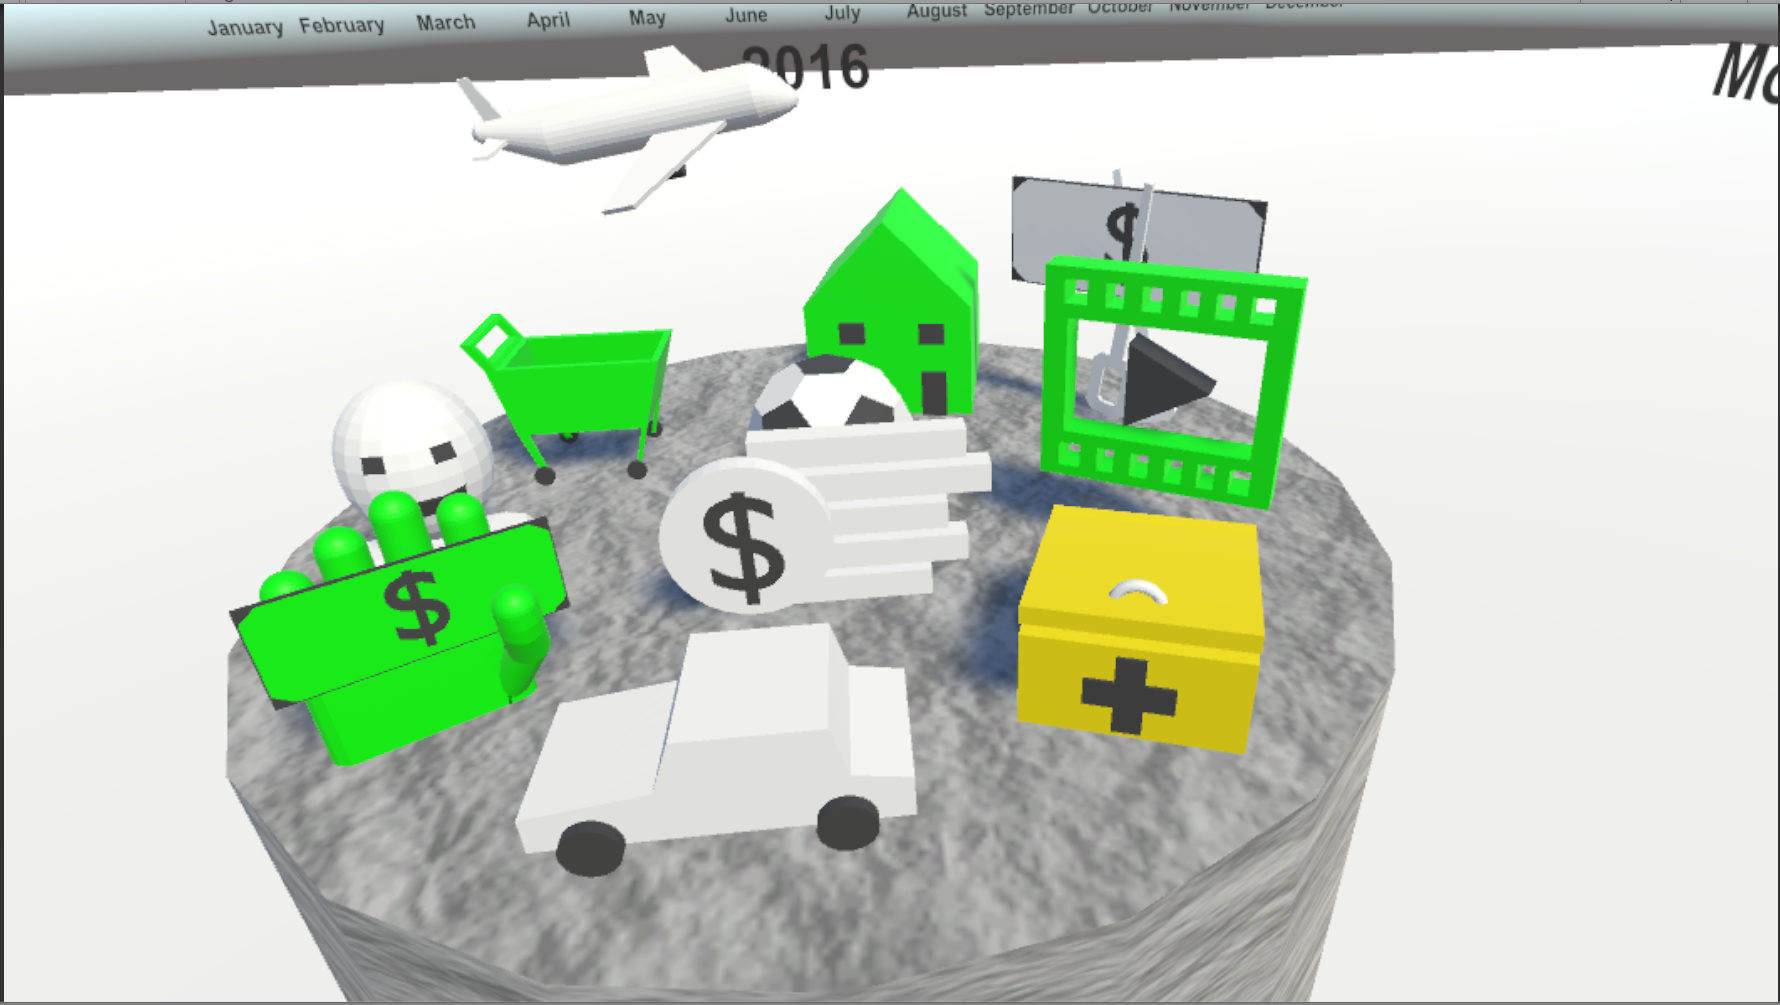
\includegraphics[width=12cm]{03_Figures/08_Development/View4_CategoriesFiltering_Loading.png}
		\caption{View 4: Categories Filtering (live in \gls{vr})}
		\label{fig:unityview4}
	\end{center}
\end{figure}


%-----------------------------------
%	SUBSUBSECTION 5
%-----------------------------------
\subsubsection{View 5: Fin. Transactions Overview}

To the right of the month overview (View 2), or opposite the year overview (View 1), the table with the list of financial transactions is positioned.

\textbf{Purpose of view:} This table provides the most important information about the financial transactions. It is not only filtered by the activated category icons from View 3, it also either display all transactions from a whole month (View 2), or if a single day had been selected, then it only displays the transactions from that specific day. The table is sorted by date which should help to have good grasp of the data. If a row has been selected, it is highlighted with blue colour to ensure the connection from the detail view (View 6) to this table can always be made.

\textbf{Possible Interaction:} Selecting a row to...
\begin{itemize}[noitemsep,nolistsep]
	\item see the full transaction details (Path 8)
\end{itemize}

\begin{figure}[h]
	\begin{center}
		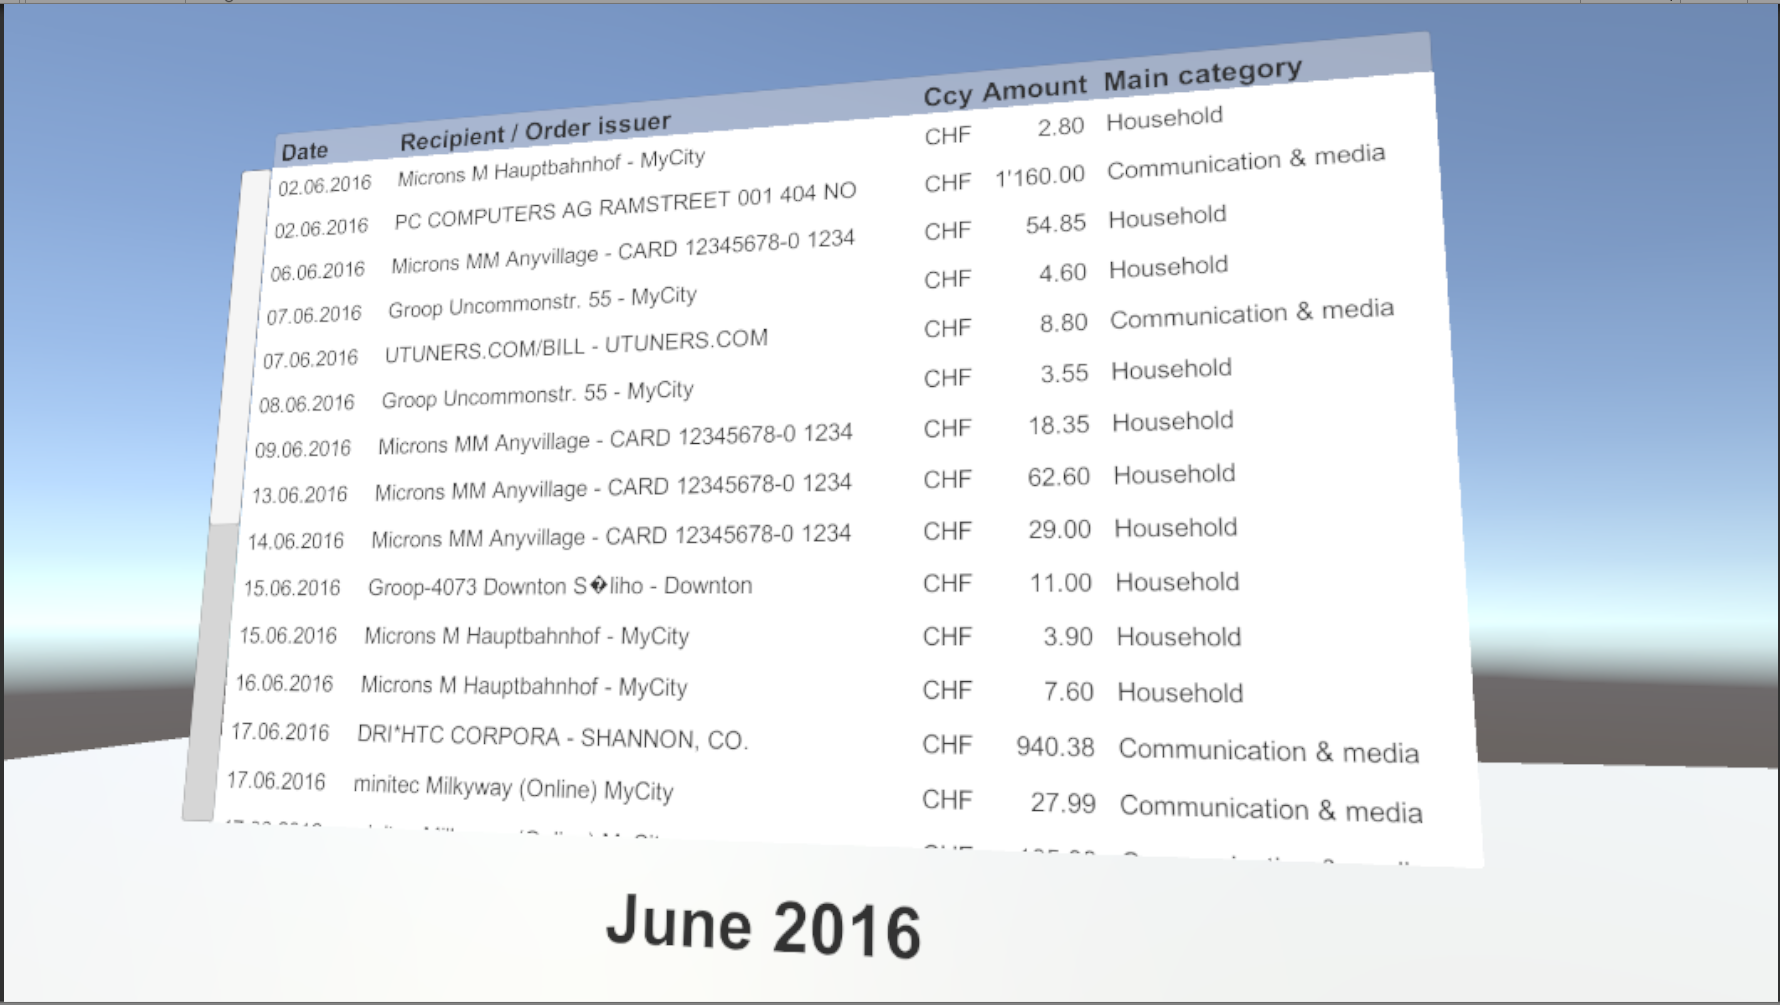
\includegraphics[width=12cm]{03_Figures/08_Development/View5_FinTransactionsOverview.png}
		\caption{View 5: Fin. Transactions Overview (live in \gls{vr})}
		\label{fig:unityview5}
	\end{center}
\end{figure}


%-----------------------------------
%	SUBSUBSECTION 6
%-----------------------------------
\subsubsection{View 6: Fin. Transaction Details}

Directly to the right of the table, the detail view is located. It is only displayed if a single transaction has been selected from the table (View 5).

\textbf{Purpose of view:} In addition to the data that had already been shown in the table to the left (View 5), additional information about the transaction is presented here. The account number as well as the account name from which the payment was made are shown, the custom booking text is displayed and also the subcategory which helps to further understand what kind of payment this was exactly. From a navigation point of view, this is the last screen and does not allow for any further navigations.

\textbf{Possible Navigation:} N/A

\begin{figure}[h]
	\begin{center}
		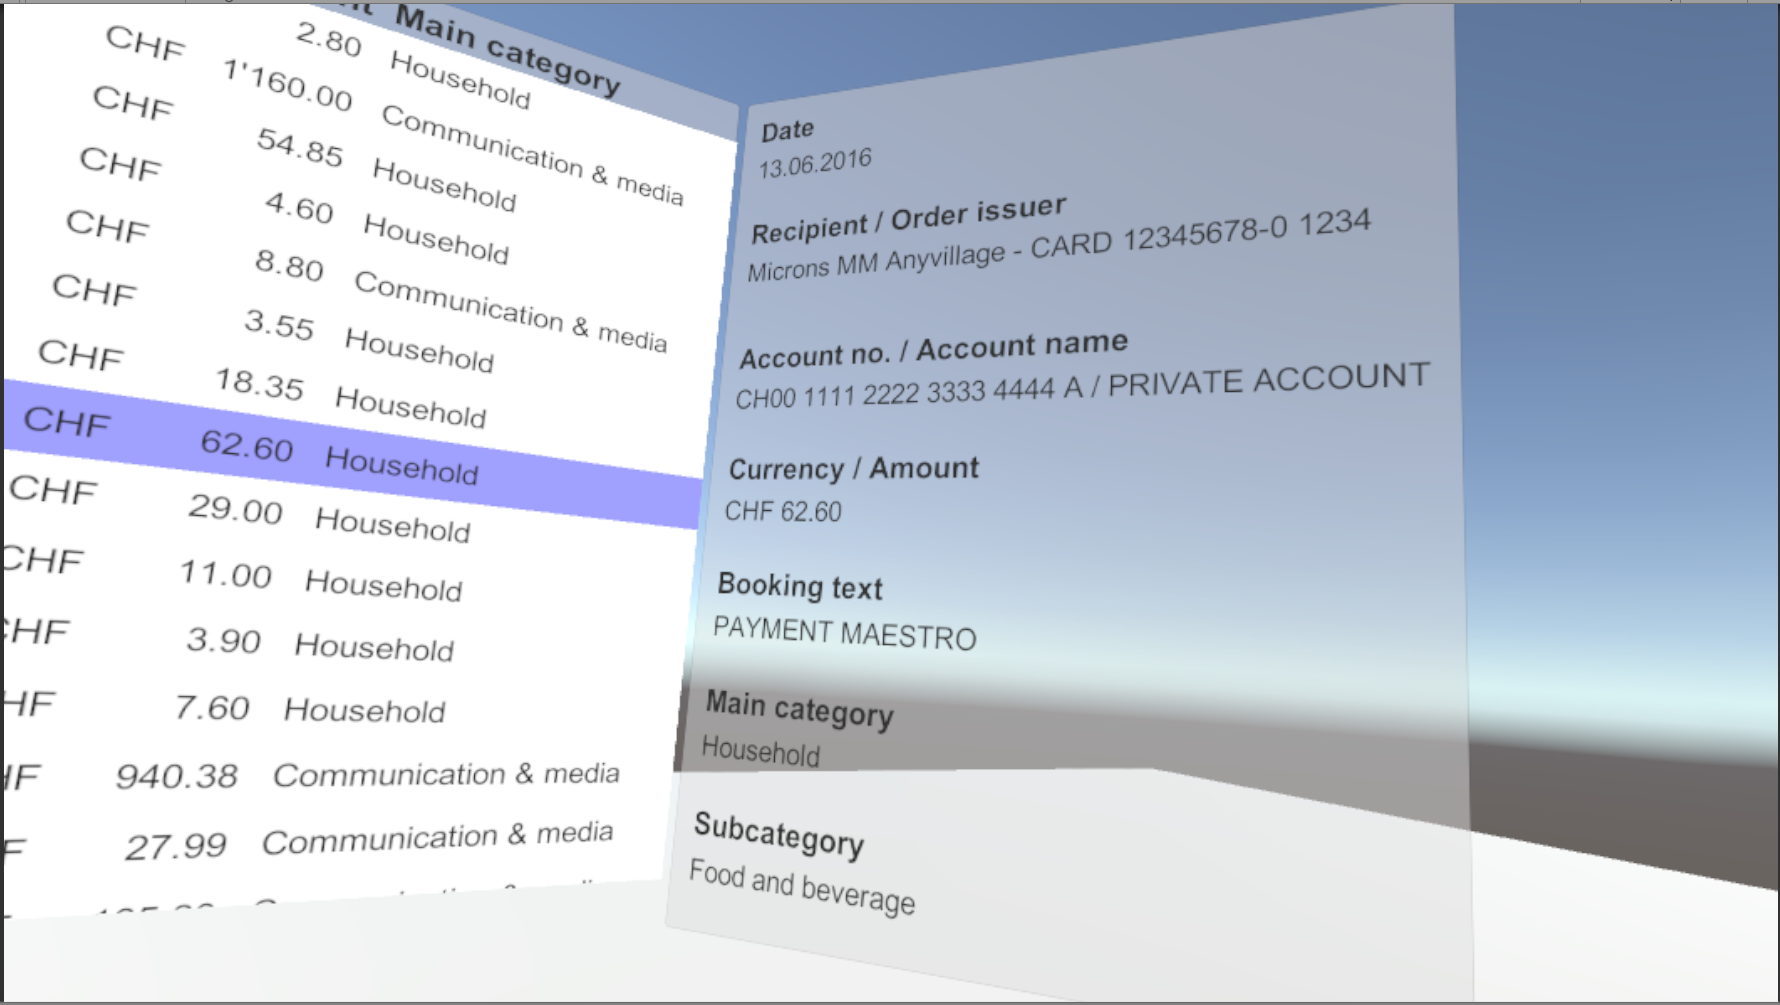
\includegraphics[width=12cm]{03_Figures/08_Development/View6_FinTransactionDetails.png}
		\caption{View 6: Fin. Transaction Details (live in \gls{vr})}
		\label{fig:unityview6}
	\end{center}
\end{figure}


%-----------------------------------
%	SUBSECTION 2
%-----------------------------------
\subsection{Interactions}

The gesture controllers themselves provide three different means of interaction with the \gls{ve}. In order to familiarize the user with these in an immersive way, upon loading the prototype application, tooltips indicate on the visualised controller which buttons us used for what. These tooltips remain visible for a limited amount of time and then disappear to not become too distractive for experienced users. Figure \ref{fig:unitypointertooltips} shows on the left side how this tooltips look like. \newline
Since the different views are rather far away from where the user is spawned, a pointer functionality has been introduced to the gesture controllers. By pressing the touchpad the pointer becomes visible and can be used as a form of an extended hand. With it, all selection functionalities can be triggered which are described in more details below. Figure \ref{fig:unitypointertooltips} shows on the right side how this pointer looks like and also how it collides with any 3D objects in the \gls{ve}.
\begin{figure}[h]
	\begin{center}
		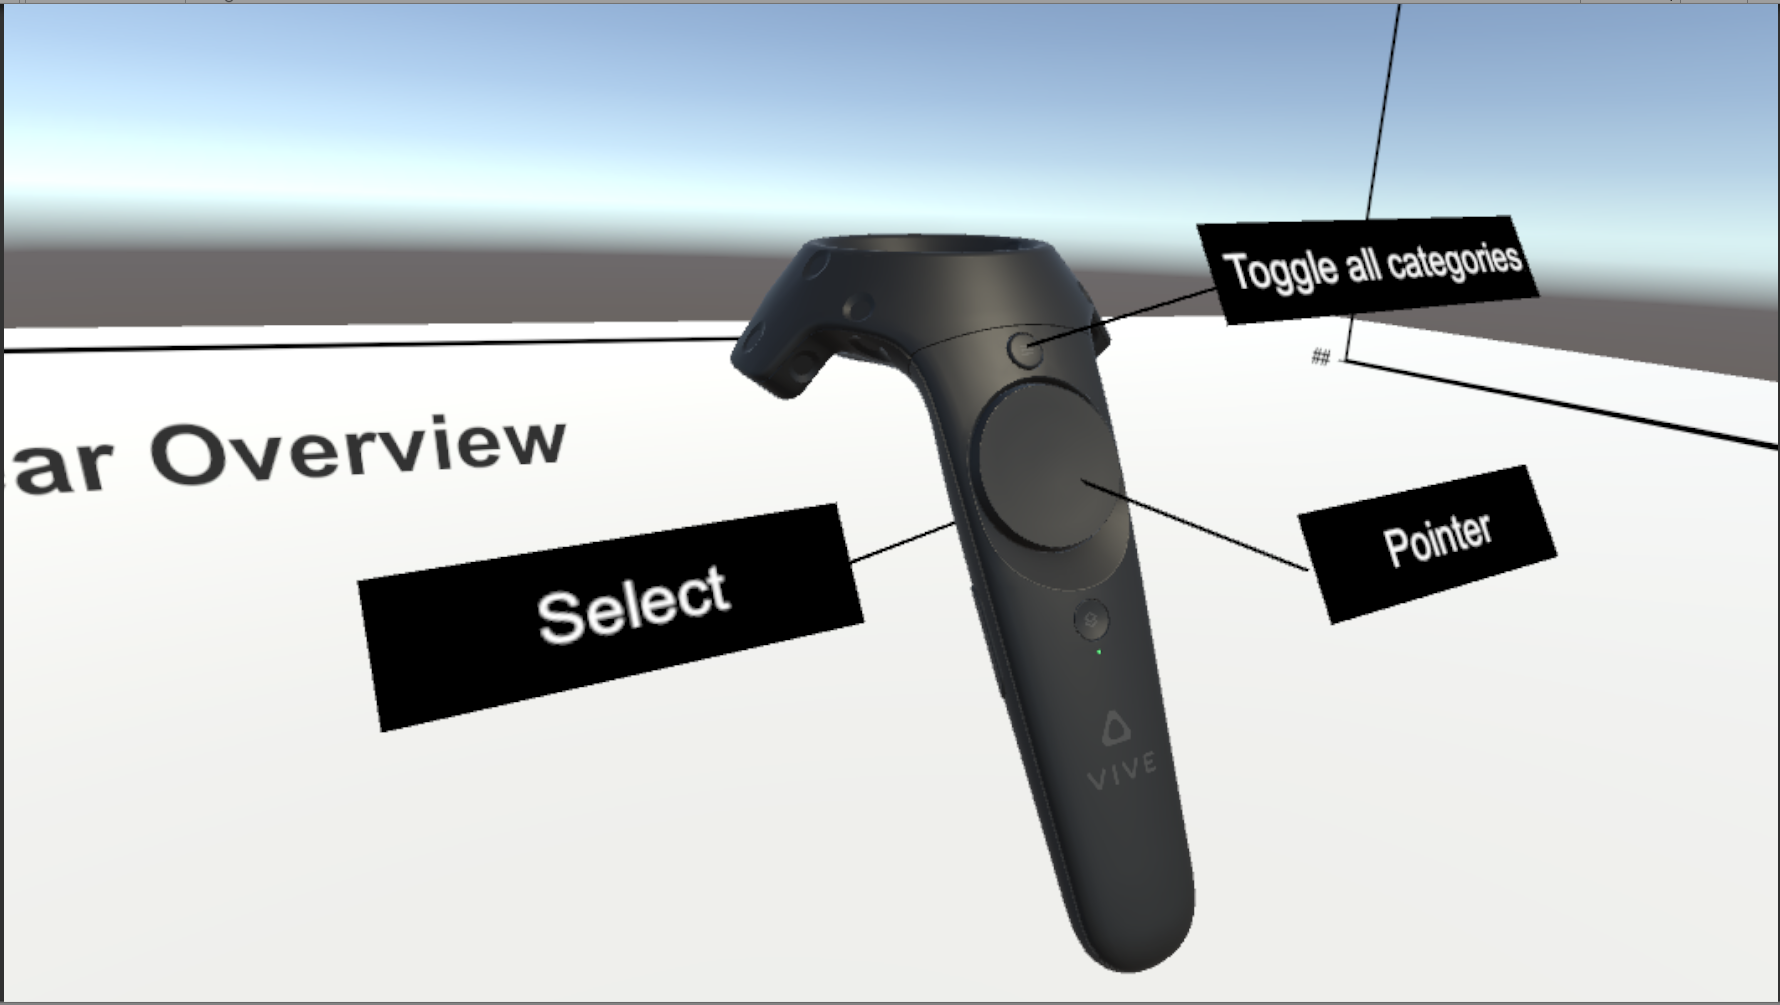
\includegraphics[width=7cm]{03_Figures/08_Development/Controller_Tooltips.png}
		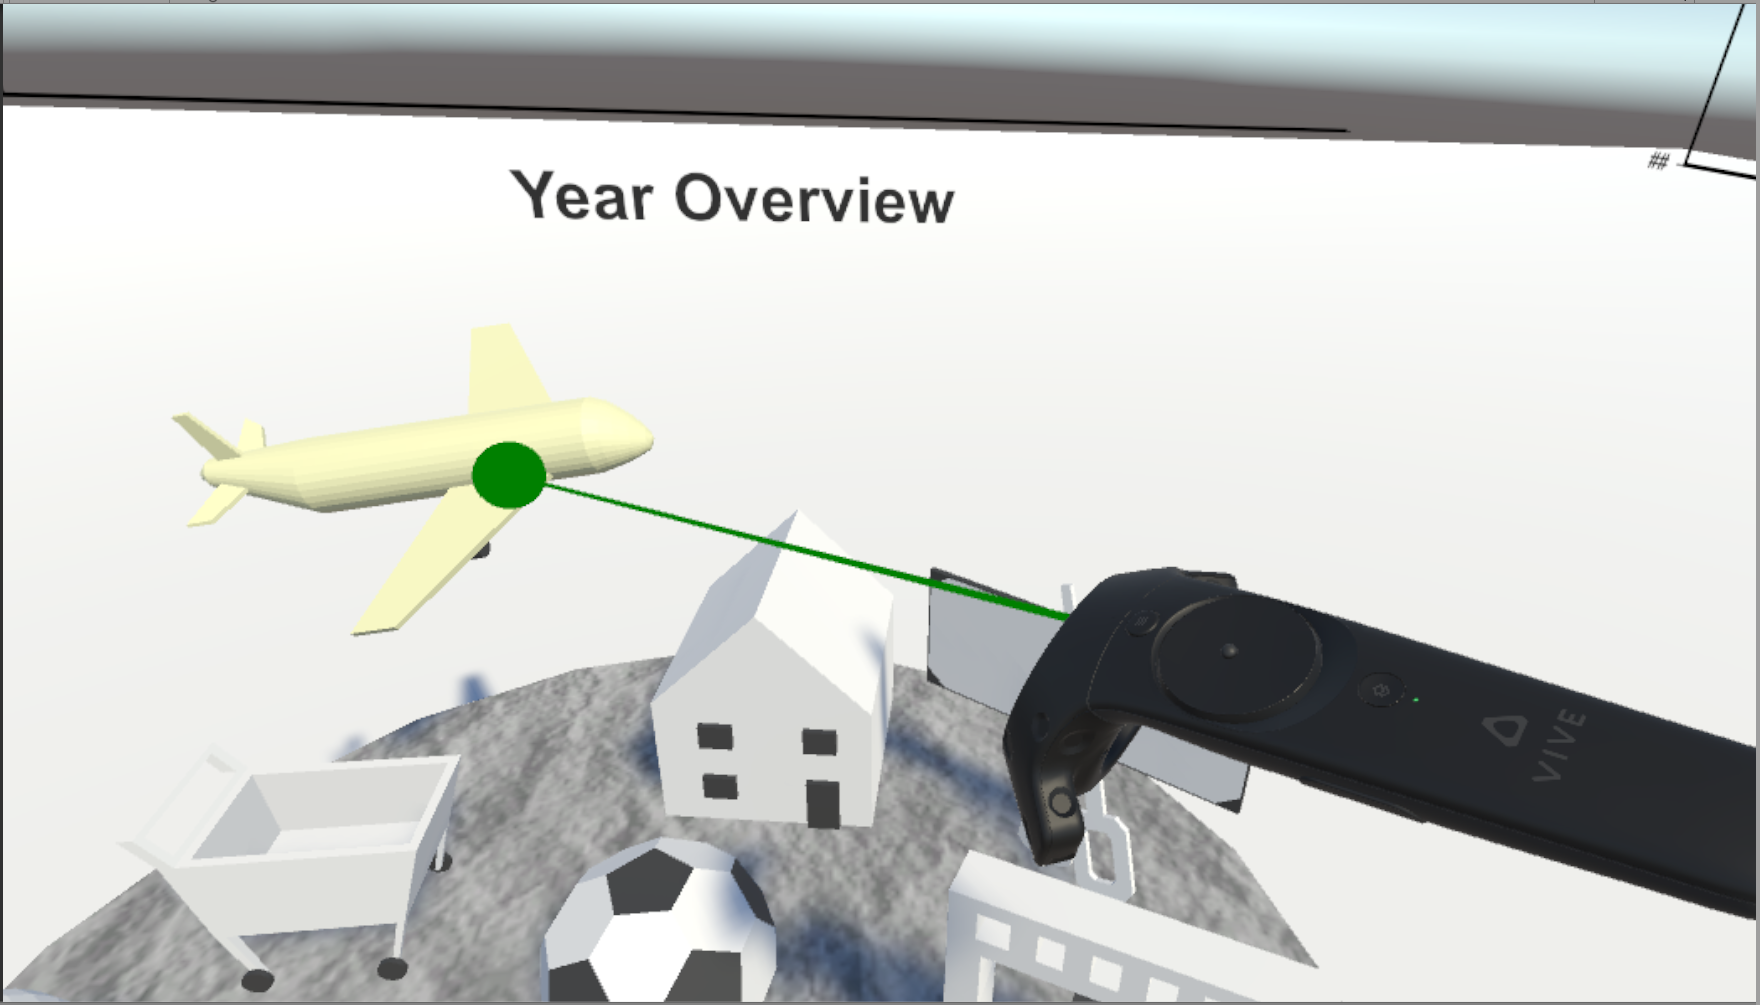
\includegraphics[width=7cm]{03_Figures/08_Development/Controller_Pointer.png}
		\caption[Gesture Controller Button Tooltips and Pointer (live in \gls{vr})]{Gesture Controller Button Tooltips (a) and Pointer (b) (live in \gls{vr})}
		\label{fig:unitypointertooltips}
	\end{center}
\end{figure}

As for the specific interactions, the first one that will automatically be triggered by the system upon starting the prototype is locating the CSV file and reading the data from it. In addition to this, by referring back to the Interaction Map in Figure \ref{fig:interactionmap}, four more interactions can be distinguished, leading up to a total of five:
\begin{itemize}[noitemsep,nolistsep]
	\item Reading in data from CSV file
	\item Selecting a year in view 3 (Path 1 and 2)
	\item Selecting a bar in a bar chart in view 1 or 2 (Path 3 and 4)
	\item Selecting a category icon in view 4 (Path 5, 6, and 7)
	\item Selecting a row in the table in view 5 (Path 8)
\end{itemize}
More detailed information about the implementation and code design of these is provided in the following sub-chapters.


%-----------------------------------
%	SUBSUBSECTION 1
%-----------------------------------
\subsubsection{Reading in data from CSV file}

The application currently only supports a single CSV file to be read in, but it can be of any name as long as it is located in the projects root folder.

\textbf{Purpose of interaction:} This interaction is automatically triggered upon starting the application in the \texttt{Start()} method of Unity, which is called on that moment when a script is enabled, just before all other methods can be called. Since this method has to be executed as one of the very first things, it is part of the \texttt{SceneManger.cs} class, which is assigned to the same empty GameObject like the SDKManager from \gls{vrtk} is. Due to this it is ensured that it is called immediately and not only when a specific GameObject is "used" for the first time.

\textbf{Implementation details:} The application looks for all \texttt{*.csv} files that exist in the root-directory of the application and takes the first one it finds. The information is read and stored in a \texttt{DataTable} out of which a \texttt{DataView} is created that can be sorted by the date of the financial transactions. Sorting a DataView works based on the name of the corresponding column that has to be defined on the very first row. Based on the sorted list, the first and last date can be read which gives an indication for how many month and year loops need to be done in order to filter and store every single. Within this loop, also the list for the Year Selection view is prepared in the \texttt{YearTable.cs} class. Since filtering is a resource-intensive task, the filtered views are stored back into DataTables and then put with their unique key (\texttt{[$<$year$>$-$<$month$>$]}) into a Dictionary: \texttt{public Dictionary<string, DataTable> dataTableDict;}. These DataTables are then later used for a better performing sub-filtering on just the individual months data-set.

%-----------------------------------
%	SUBSUBSECTION 2
%-----------------------------------
\subsubsection{Selecting a year}

\textbf{Purpose of interaction:} Although the latest year from the data-set is automatically pre-selected for viewing and filtering, depending on the size of the data set there might also be data for previous years that the user should be able to look at. With the simple Year Selection view, that is dynamically populated during the CSV import, the user has the possibility to change the year in a very convenient way. See also Figure \ref{fig:unityview3} that shows how the Year Selection view looks like.

\textbf{Implementation details:} As part of the year-loop inside the \texttt{SceneManager.cs} class, the code snippet in Listing \ref{lst:csharpaddingyearstotable} is executed once for every year. It looks for a GameObject that has the \texttt{YearTable} script assigned to it, which in this case is the frame of the whole view in which then multiple year objects can be displayed.
\begin{lstlisting}[caption={SceneManager.cs : Adding years to the YearTable}, label={lst:csharpaddingyearstotable}]
// Add the current year to the year selection table
YearTable yearTable = GameObject.FindObjectOfType<YearTable>();
yearTable.AddYearToTable(currYear);
\end{lstlisting}
Inside the \texttt{YearTable.cs} class, the method \texttt{AddYearToTable(int year)} is called which creates a new instance of the GameObject that represents an entry in the table and has been stored as a prefab. This allows to seamlessly create new objects that have the exact same configuration, and it further reduces the memory load since only instances are created and not complete new objects. This new GameObject is then set as a child of the class itself and thus the "frame" where all the rows are hold together. If the list was empty when the new year was added, its colour is changed to indicate that this row has been preselected. All future entries will not have this modification and thus remain with a white background colour. A reference to the \texttt{Image} whose colour was changed has to be stored in the \texttt{SceneManager.cs} class to make sure that when a different year is selected, the \texttt{SceneManager.cs} still remembers which \texttt{Image} was selected before and therefore reset its colour back to white. Listing \ref{lst:csharpyeartable} shows in a \textbf{simplified} way how this logic looks like in the \texttt{YearTable.cs} class.
\begin{lstlisting}[caption={YearTable.cs : Simplification of adding a new year to the table}, label={lst:csharpyeartable}]
public void AddYearToTable(int year) {
  Year newYearRow;
  // Instantiate new Year
  newYearRow = Instantiate(yearPrefab);
  newYearRow.transform.SetParent(yearTableFrame);
  // Set the label
  newYearHolder.yearText.text = year.ToString();
  if (yearRows.Count == 0) {
     // First year we add, therefore pre-selected it
     Image firstYearImg = newYearRow.GetComponent<Image>();
     firstYearImg.color = SceneManager.Instance.selectedRowColor;
     // store in scenemanager for proper de-selection later
     SceneManager.Instance.selectedYearRowImg = firstYearImg;
  }
  // Add the bar to the list
  yearRows.Add(newYearRow);
}
\end{lstlisting}


%-----------------------------------
%	SUBSUBSECTION 3
%-----------------------------------
\subsubsection{Selecting a bar in a bar chart}

\textbf{Purpose of interaction:} By default the user starts with the Year Overview where possible  one or more months have expenses that exceeded the pre-defined threshold. The most intuitive way to then select this specific month (or the specific day in case of the Month Overview) is by actually pointing at it and then selecting it. When a month has been selected, its corresponding Month Overview will be displayed as well as the table is updated with a list of financial transactions. How the selection can look like is shown in Figure \ref{fig:unitybarselection} where the bar that is pointed at gets slightly opaque. If this bar then is actually selected, it starts flashing so it is easily visible for which bar the other views display their data now.
\begin{figure}[h]
	\begin{center}
		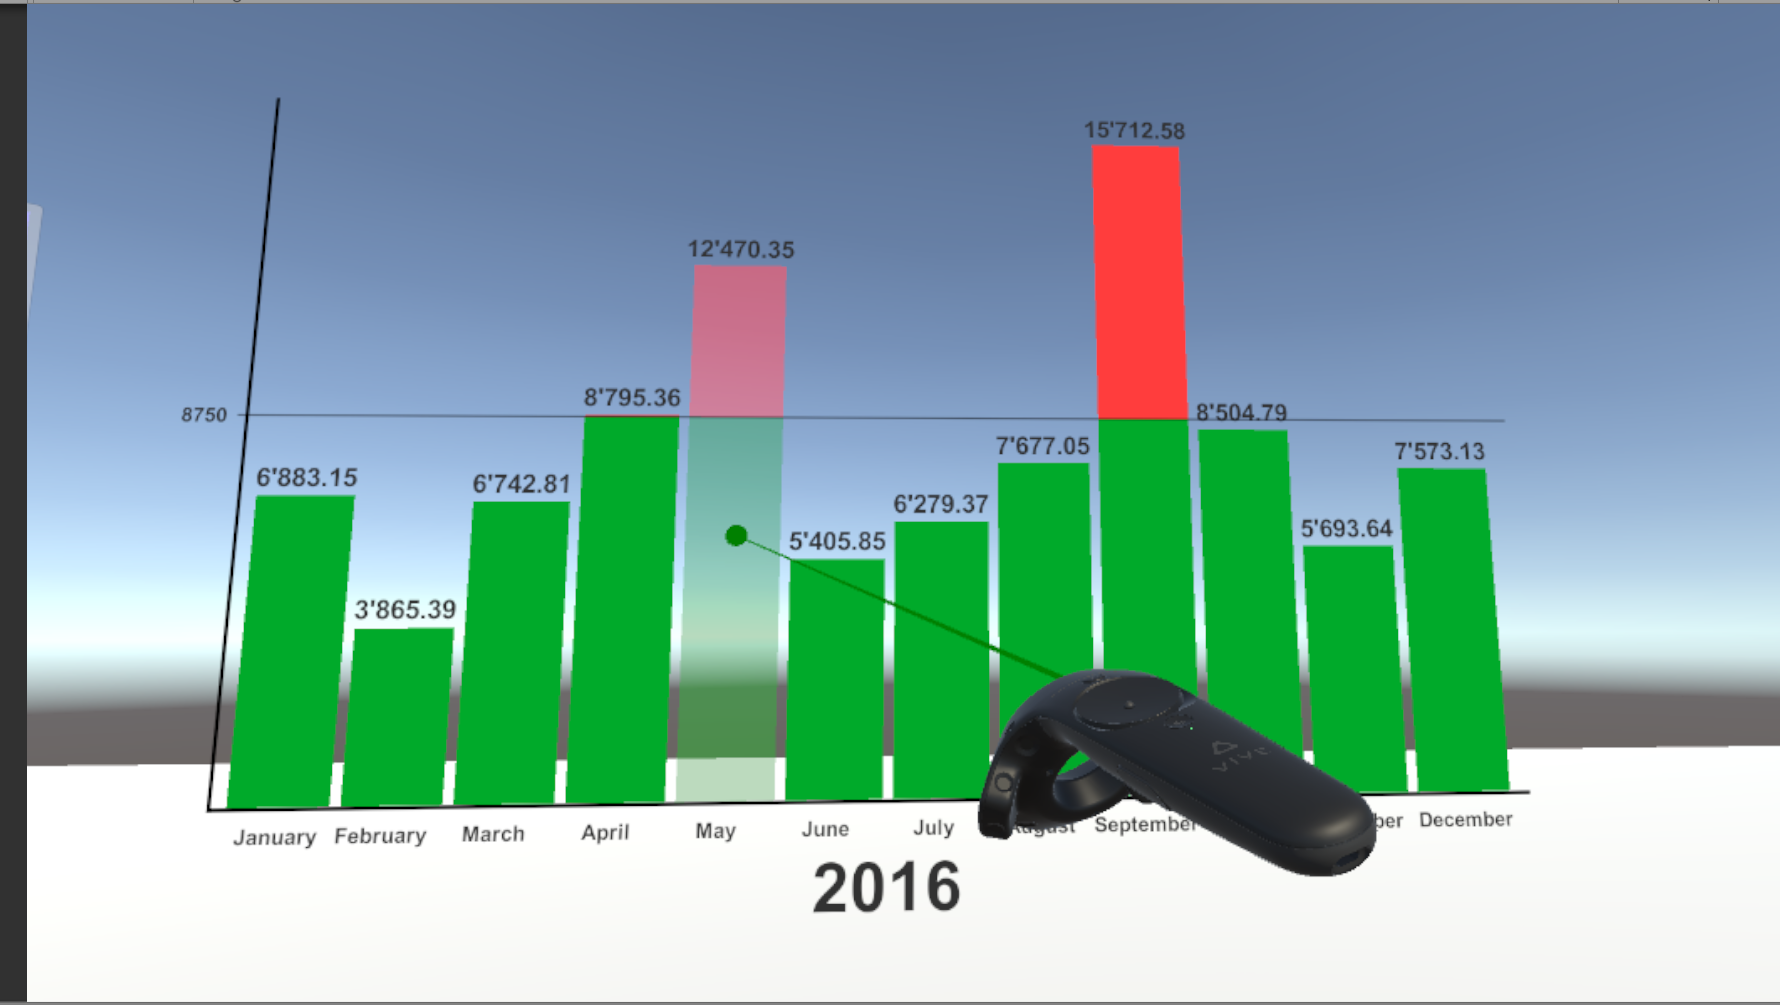
\includegraphics[width=12cm]{03_Figures/08_Development/Bar_Selection.png}
		\caption{Selecting a bar with the Gesture Controller Pointer (live in \gls{vr})}
		\label{fig:unitybarselection}
	\end{center}
\end{figure}

\textbf{Implementation details:} Each bar of the two charts has the \texttt{ChartBarClick.cs} script attached to it which is responsible for all direct interaction with it. It consists of three methods: \texttt{StartTouching()}, \texttt{StopTouching()}, and \texttt{StartUsing()}. The first two are to make sure that the bar becomes slightly opaque upon "touching" it and then returns to its normal colour when the "touching" ends. The \texttt{StartUsing} method first checks to which chart this bar belongs, stops any other flashing bars if existing, starts flashing the selected bar, updates the information about the selected month/day in the \texttt{SceneManager.cs} and finally triggers the following method: \newline
\texttt{SceneManager.Instance.updateSelection(label);} The \texttt{label} in this case can either be a numeric value of the selected day (e.g. "5"), or a string value of the selected month (e.g. "May"). The steps that are executed as part of the \texttt{updateSelection()} are rather complicated. Figure \ref{fig:unityupdateselection} should help to illustrate what exactly happens alongside the below high-level description.
\begin{enumerate}[noitemsep,nolistsep]
	\item When clicking on a bar, the \texttt{ChartBarClick.cs} calls the \texttt{updateSelection()} method from the \texttt{SceneManager.cs} class
	\item This first resets the DetailView with \texttt{updateDetailView(null);}
	\item Then it starts a Coroutine (i.e. flow control is cooperatively passed between itself and the game engine)
	\item The Coroutine opens a 2nd Thread for the CPU intensive work to not not block the GameEngine and prevent the \gls{ve} from freezing for a few seconds
	\item The 2nd Thread filters all data, updates the ArrayLists and caches the results
	\item Meanwhile, the Coroutine checks if the Thread is still running and gives temporary flow control to the GameEngine
	\item When the Thread has ended, the Coroutine continues with \texttt{updateBarCharts();}
	\item Then, also the table is updated with \texttt{updateTable();}
	\item Both methods now use the cached data that had been created by the \texttt{ThreadedWork()}
\end{enumerate}
\begin{figure}[h]
	\begin{center}
		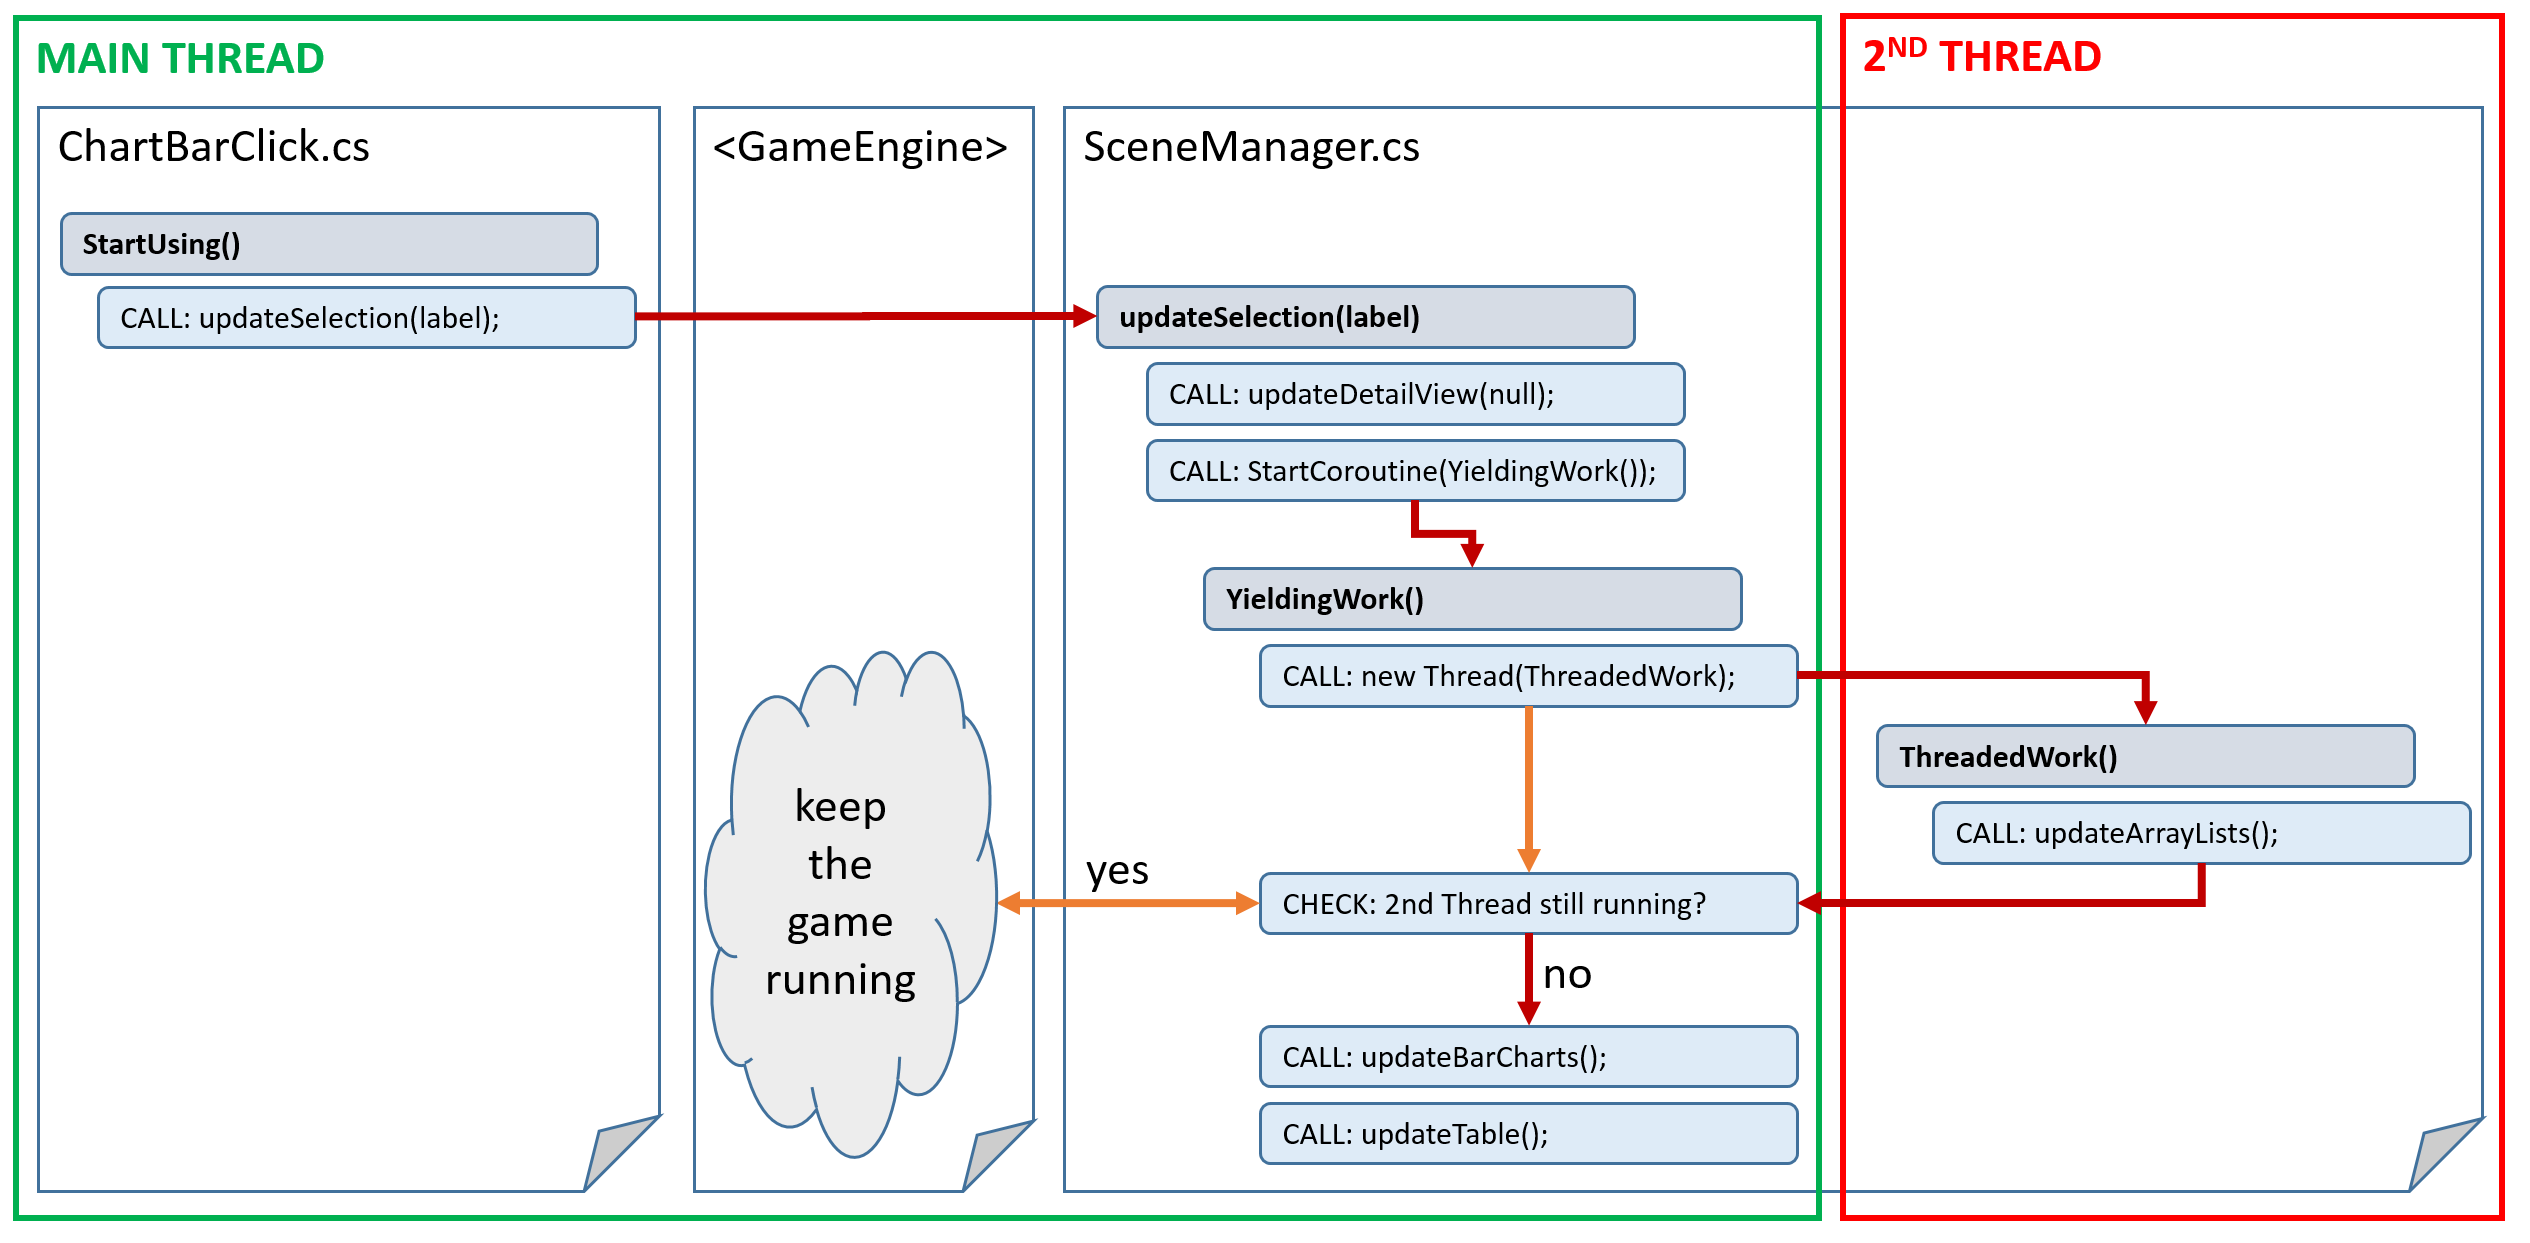
\includegraphics[width=14cm]{03_Figures/08_Development/UpdateSelection.png}
		\caption{Illustration of updateSelection() workflow}
		\label{fig:unityupdateselection}
	\end{center}
\end{figure}
This implementation with a Coroutine that calls a 2nd Thread was necessary to avoid freezing in the whole \gls{ve} for several seconds during the very CPU intensive task of filtering and preparing the datasets. It further mitigates the risk now of potential motion-sickness that could occur in such situations. \newline
Some additional challenges came up with this approach though, as certain functions are only allowed (by the Unity Game Engine) to be called from the \textbf{Main Thread} and not from a 2nd Thread. This required that the output of these function calls had to be generated before calling the 2nd Thread and then passing them on into it, respectively making it available to it inside the class itself.


%-----------------------------------
%	SUBSUBSECTION 4
%-----------------------------------
\subsubsection{Selecting a category icon}

\textbf{Purpose of interaction:} This covers one of the main flaws of the traditional solution to represent financial transactions to users: In addition to just displaying the data of a single category, they can be combined in any possible combination  and thus can give an unique insight into ones personal expenses. 

\textbf{Implementation details:} When looking at Figure \ref{fig:unityupdateselection} from the previous interaction, the one for selecting a category is almost the same. The only difference is the beginning as the Coroutine is not triggered by the \texttt{updateSelection()} method, but by either \texttt{addGameObjectToCategoryFilter()} or \texttt{removeGameObjectFromCategoryFilter()} where a reference to the \texttt{CategoryIconClick.cs} is also passed on (or an ArrayList in case all category icons are de-/selected). To make the user more aware of the fact that a loading process is ongoing, as soon as the Coroutine is started, the corresponding category object is coloured in \textbf{yellow}, as also shown in Figure \ref{fig:unityview4}. When the Coroutine ended, the colour of the category object is either changed to green (activated) or white (deactivated). The decision for this was made in accordance to \gls{mdg} 1 which requires a high interactivity with tightly coupled actions/reactions. While the updated data is only shown in a very short amount of time after it had been cashed, this third state at least gives immediate feedback to the user that his input was registered and something is going on.


%-----------------------------------
%	SUBSUBSECTION 5
%-----------------------------------
\subsubsection{Selecting a row in the table}

\textbf{Purpose of interaction:} The table with a list of financial transactions already gives a good overview to the user about the individual transactions that happened on the selected month or day. But sometimes this information is still not enough and more details are required. Similar to the approach of \cite{CodeScience2015}, a dedicated view for the detail information is defined. When a row in the table is selected, it is highlighted accordingly so that it at all times is clear from which entry in the table the details are shown now. This is also illustrated in Figure \ref{fig:unityview6}.

\textbf{Implementation details:} Like the \texttt{CategoryIconClick.cs} for the category objects, or the \texttt{ChartBarClick.cs} for the chart bars, there also is a \texttt{TableRowClick.cs} class for when one of the rows in the table has been selected. Since the \texttt{Row.cs} class that is used to represent the individual rows in the table already has all detail information in it, the \texttt{updateDetailView()} method \texttt{SceneManager.cs} simply has to be called with a reference to itself. After checking that the provided reference is not \texttt{null} (which would cause the DetailView to be hidden), all the details from the row object are extracted and shown in the view.


%----------------------------------------------------------------------------------------
%	SECTION 5
%----------------------------------------------------------------------------------------

\section{Conclusion}

In this chapter, a summary of challenges that occurred and had to be overcome, as well as new findings during the development is presented. Like in every software development project, new results and insights are gained while working on it, which is a key part of continuous improvements of a design. For this prototype application, many new products and systems had to be learned and used in order to bring the best possible value to the development. In the following sub-chapters, some of the highlights are summarized.


%-----------------------------------
%	SUBSECTION 1
%-----------------------------------
\subsection{Unity 3D and C\#}

While familiar with the programming language Java, C\# was not too difficult to adapt to. But even then it had some unique features that can be challenging at times or at least require some further research in order to understand how this works in this programming language. Some examples are listed here:
\begin{itemize}[noitemsep,nolistsep]
	\item There is no real difference between \texttt{String} and \texttt{string} (upper-/lower-case)
	\item A \texttt{HashMap} from Java is a \texttt{Dictionary} in C\#
	\item There is no \texttt{Date} object in C\#, only \texttt{DateTime} exists
	\item Additional core-features from .NET have to be manually added by enabling the corresponding \texttt{*.dll}
	\item Getter and Setter methods are not explicitly required as they are Auto-Implemented Properties
\end{itemize}
A much bigger challenge than C\# however was Unity 3D itself as this was absolutely new. Online tutorials for development with \gls{vr} existed, but mostly were for much older versions of Unity and thus no longer applicable. Especially since in Unity 3D version 5.4 native support for OpenVR was provided that would simplify man programming tasks that had to be tediously done in version 5.3 and earlier. This sooner or later lead to the discovery of \gls{vrtk}.


%-----------------------------------
%	SUBSECTION 3
%-----------------------------------
\subsection{\gls{vrtk}}

\gls{vrtk} massively simplifies the development of \gls{vr} applications in Unity 3D. It is a collection of useful scripts and concepts that help building \gls{vr} applications. There is an excellent documentation available and the

excellent documentation https://vrtoolkit.readme.io/
yoututbe tutorials
shipped with many example scenes

%-----------------------------------
%	SUBSECTION 2
%-----------------------------------
\subsection{Blender}





%% IDEA FOR PROTOTYPE

% - Start with a small table on which a house etc is visualized. floating above is year (+month)
% + Each object represents one category from the financial expenses.
% - maybe size indicates the overall amount?
% - The colours depends on the difference between my planned expenses (or average expenses) and the actual expenses. less = green, about the same = yellow-(green-)ish, slightly above = orange, above = red.
% - By clicking on one of the objects, it gets highlighted and a line-chart appears showing the expenses
% A) show individual transactions for the given month up until the threshold
% B) show individual months until the threshold (+forecast?)
% - show multiple lines for the different sub-categories (enable/disable) plus the total
% - clicking on an entry of the line chart displays details about transaction (amount, location), or the month (amount) in an overlay
% - switching between single-month and year view by... using the touchpad (up/down clicks)
% - navigating through months/years by... a using the touchpad! (left/right clicks)
% - resetting the view to start by... clicking on the select button

% - maybe outside as rotating rings: the individual bank accounts?
